\chapter[Strelka2Pass and FreeBayesSomatic publication]{Custom workflows to improve joint variant calling from multiple related tumour samples: FreeBayesSomatic and Strelka2Pass}
\label{ch:appendixManuscript}

This appendix contains the manuscript published at \textit{Bioinformatics} in an non journal style format with the supplementary methods and figures. It can also be found at \href{https://doi.org/10.1093/bioinformatics/btab606/6361543}{10.1093/bioinformatics/btab606/6361543} for a paper style version.
\vspace{1em}
\hrule
\vspace{2em}

{\Large \textbf{Hollizeck S.$^{1,2}$, Wong S.Q.$^{1,2}$, Solomon B.$^{1,2}$, Chandrananda D.$^{1,2,*}$, and Dawson S-J.$^{1,2,3,*}$}}

{
$^1$ Peter MacCallum Cancer Centre, Melbourne 3000, Victoria, Australia\\
$^2$ Sir Peter MacCallum Department of Oncology, University of Melbourne, Melbourne 3000, Victoria, Australia\\
$^3$ Centre for Cancer Research, University of Melbourne, Melbourne 3000, Victoria, Australia\\
\vspace{0.5em}
$^*$ D.C and S.J.D are co-senior authors and contributed equally to this article
}

{\small
Received on 27-Jan-2021; revised on 13-Jul-2021; accepted on 12-Aug-2021
}

{\Large \textbf{Abstract}}
\vspace{-2em}
\paragraph{\textbf{Summary:}} This work describes two novel workflows for variant calling that extend the widely used algorithms of Strelka2 and FreeBayes to call somatic mutations from multiple related tumour samples and one matched normal sample. We show that these workflows offer higher precision and recall than their single tumour-normal pair equivalents in both simulated and clinical sequencing data.
\vspace{-2em}
\paragraph{\textbf{Availability and Implementation:}} Source code freely available at the following link:
\href{https://atlassian.petermac.org.au/bitbucket/projects/DAW/repos/multisamplevariantcalling}{\nolinkurl{https://atlassian.petermac.org.au/bitbucket/projects/DAW/repos/multisamplevariantcalling}}
and executable through Janis (\href{https://github.com/PMCC-BioinformaticsCore/janis}{\nolinkurl{https://github.com/PMCC-BioinformaticsCore/janis}}) under the GPLv3 licence.
\vspace{-2em}
\paragraph{\textbf{Contact:}} \href{Dineika.Chandrananda@petermac.org}{Dineika.Chandrananda@petermac.org}, \href{Sarah-Jane.Dawson@petermac.org}{Sarah-Jane.Dawson@petermac.org}
\vspace{-2em}
\paragraph{\textbf{Supplementary information:}} Supplementary data are available at \textit{Bioinformatics}
online.


%if we want to make it more journal style, we use 2 columns, but it requires a bit of tweaking for the formulas
%\begin{multicols}{2}

\section{Introduction}
Joint variant calling methods are routinely used to call germline variants by leveraging population-wide information across multiple related samples \parencite{DePristo2011,Toptas2018}. This concept is also advantageous for somatic variant calling to potentially overcome the challenges of spatial heterogeneity and low tumour purity. However, there is a critical lack of robust algorithms that allow multi-sample somatic calling. Most studies still rely on variant calling of separate tumour-normal pairs, subsequently combining the results across a sample cohort \parencite{Hu2019, Leong2018, Wang2018}.

There are two major pitfalls for combining variants called from individual tumour samples. First, it is very difficult to differentiate between a false negative result due to "missing data" versus the true absence of a variant. Second, there is limited sensitivity for low allele frequency variants thus, decreasing the ability to detect minor clones, particularly in samples with low tumour purity.

Currently, only three algorithms claim to have the functionality to jointly analyse multiple samples: multiSNV \parencite{Josephidou2015}, SuperFreq \parencite{Flensburg2020}, and Mutect2 \parencite{Benjamin2019}, each presenting different limitations. For instance, multiSNV cannot call indels and along with SuperFreq, is not optimised for analysis of deep coverage whole-genome sequencing (WGS) data. Mutect2 has previously been shown to be disadvantageously conservative as well as computationally inefficient \parencite{Chen2020a}.

To enable highly sensitive, fast and accurate variant detection from multiple related tumour samples, we have developed joint variant calling extensions to two widely used single-sample algorithms, FreeBayes \parencite{Garrison2012} and Strelka2 \parencite{Kim2018}. Using both simulated and clinical sequencing data, we show that these workflows are highly accurate and can detect variants at much lower variant allele frequencies than commonly used methods.

\section{Materials and methods}
\subsection{FreeBayesSomatic workflow}
The original FreeBayes algorithm can jointly evaluate multiple samples but routinely it does not perform somatic variant calling on tumour-normal pairs. We introduce FreeBayesSomatic which allows concurrent analysis of multiple tumour samples by adapting concepts from SpeedSeq \parencite{Chiang2015} which differentiates the likelihood of a variant between tumour and normal samples instead of imposing an absolute filter for all variants called in the normal. Hence, for each genotype (GT) at SNV sites, FreeBayesSomatic first calculates the difference in likelihoods (LOD) between the normal (\autoref{A:eq:01}) and the tumour (\autoref{A:eq:02}) samples genotype likelihoods (GL) with g$_{0}$ describing the reference genotype.


\begin{align}
\text{LOD}_{\text{normal}} &= \max_{g_i \in \text{GT}} \left( \text{GL}(g_0) - \text{GL}(g_i) \right) \label{A:eq:01}\\
\text{LOD}_{\text{tumour}} &= \min_{s \in \text{Samples}} \left( \min_{g_i \in \text{GT}} \left( \text{GL}_s(g_i) - \text{GL}_s(g_0) \right) \right) \label{A:eq:02}\\
\text{somaticLOD} & := \left( \text{LOD}_{\text{normal}} \geq 3.5 \land \text{LOD}_{\text{tumour}} \geq 3.5 \right) \label{A:eq:03}
\end{align}

Next, the variant allele frequencies (VAF) in both the tumour and the normal samples are compared at each site.


\begin{align}
\text{VAF}_{\text{tumour}} &= \max_{s \in \text{Samples}} ( \text{VAF}_s) \label{A:eq:04}\\
\text{somaticVAF} & := \left( \text{VAF}_{\text{normal}} \leq 0.001 ~\lor \right. \nonumber \\
 & \left. ( \text{VAF}_{\text{tumour}} \geq 2.7 \cdot \text{VAF}_{\text{normal}}) \right) \label{A:eq:05}
\end{align}

A variant is classified as somatic when both somaticLOD as well as somatic VAF pass the criteria somaticLOD (\autoref{A:eq:03}) and somaticVAF (\autoref{A:eq:05}).

The thresholds chosen for both LOD and VAF calculations were previously fitted by the blue-collar bioinformatics workflow for the DREAM synthetic 3 dataset using the SpeedSeq likelihood difference approach \parencite{Chapman2020} and were selected to identify high confidence variants.

\subsection{Strelka2Pass workflow}
In contrast to FreeBayes, whilst Strelka2 has a multiple-sample mode for germline analysis and tumour-normal pair somatic variant calling capabilities, it cannot jointly analyse multiple related tumour samples. We enable this feature by adapting a two-pass strategy previously used for RNA-seq data \parencite{Veeneman2015}. First, somatic variants are called from each tumour-normal pair. All detected variants across the cohort are then used as input for the second pass of the analysis where we re-iterate through each tumour-normal pair but assess allelic information for all input genomic sites.

The method re-evaluates the likelihood of each variant, by integrating every genotype from each tumour-normal pair. This step can "call" a variant ($v$) in a sample that initially did not present enough evidence to pass the Strelka2 internal filtering using two conditions: 1) if this variant was called as a proper "PASS" by Strelka2 in any other tumour sample, or 2) if the integrated evidence for this variant across all tumour-normal pairs reached a sufficiently high level. The second condition was based on the somatic evidence score (SomEVS) reported by Strelka2, which is the logarithm of the probability of the variant $v$ being an artefact.

\begin{equation}
p_{error}(v) = 10^{\left( \frac{-\text{SomEVS}(v)}{10} \right)} \label{A:eq:06}
\end{equation}

While the germline sample is shared between all processes, we can approximate these individual probabilities as being independent, since one variant calling process is agnostic of the other. Hence, we derive the following:

\begin{equation}
p_{error}(v_{s_1},v_{s_2},\ldots,v_{s_n}) = \prod_{s \in \text{Samples}} p_{error}(v_{s}) \label{A:eq:07}
\end{equation}

And therefore:

\begin{equation}
\text{SomEVS}(v_{s_1},v_{s_2},\ldots,v_{s_n}) = \sum_{s \in \text{Samples}} \text{SomEVS}(v_{s}) \label{A:eq:08}
\end{equation}

This allows the summation (\autoref{A:eq:08}) of the SomEVS score across all supporting variants to assign a "PASS" filter, if it reached a joint SomEVS score threshold. This threshold can be set by the user and is 20 by default, which corresponds to an estimated error rate of 1\%. These "recovered" variants need to pass a set of additional quality metrics related to depth of coverage, mapping quality and read position rank sum score.

As an additional improvement, we also built multiallelic support into Strelka2 which originally only reports the most prevalent variant at a specific site. Within the two-pass analysis, we reconstruct the available evidence for a multiallelic variant at a called site from the allele-specific read counts and report the minor allele at this site, if there is sufficient support from other samples. This method allows recovery of minor alleles only if another sample has this variant called by Strelka2, as SomEVS scores are not available for minor alleles.

\section{Validation}

\begin{figure*}[!ht]
\centering
  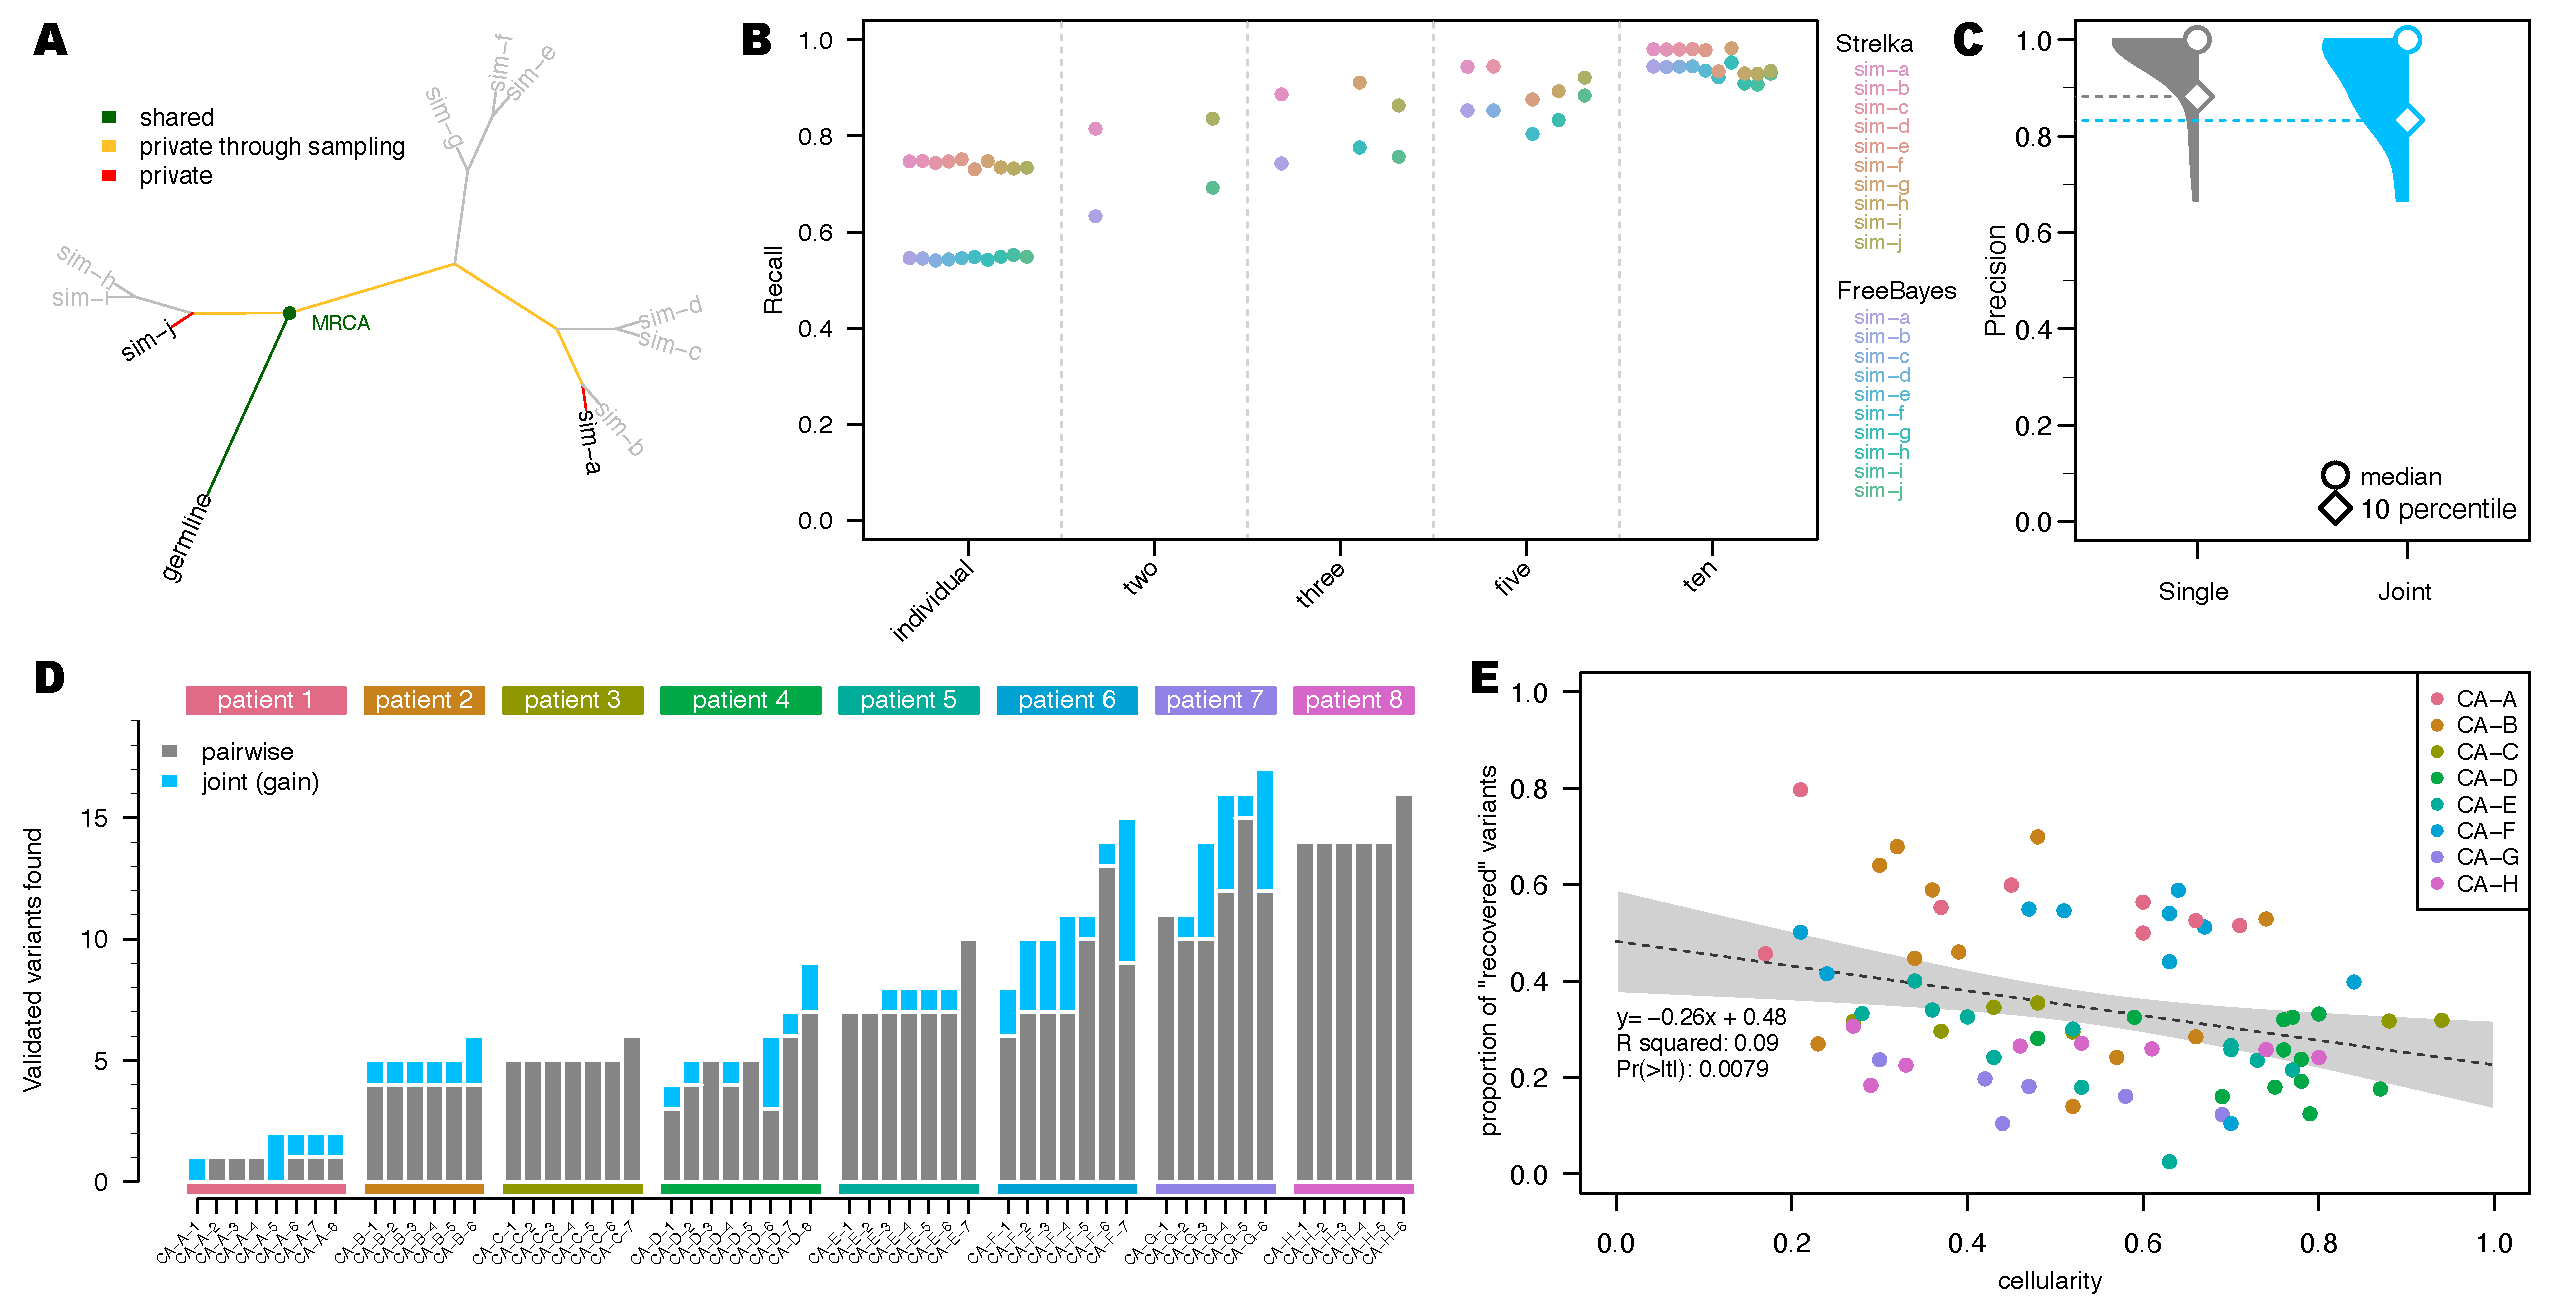
\includegraphics[width=\textwidth]{Appendices/Variantcalling/Figure_1}\vspace*{-12pt}
  \caption[Comparison of joint multi-sample variant calling and single tumour-normal paired calling methods]{Comparison of joint multi-sample variant calling and single tumour-normal paired calling methods; A) Simulated phylogeny highlighting two samples with high evolutionary distance (sim-a and sim-j) where MRCA denotes the most recent common ancestor. B) Recall estimates of FreeBayes and Strelka2, run in individual tumour-normal paired and joint calling configurations using two (sim-a and sim-j), three (sim-a, sim-g and sim-j), five (sim-a, sim-c, sim-f, sim-h and sim-j) and all ten tumour samples. C) Precision of Strelka2 and D) Number of variants called by Strelka2 run in both tumour-normal paired (grey) and added with joint calling configurations (blue), which have been validated by targeted amplicon sequencing (TAS). E) Correlation between cellularity and proportion of variants found only with joint calling using Strelka2Pass for clinical samples; grey area shows the "$95\%$" confidence interval for the linear model fit (dotted line).}\label{A:fig:01}
\end{figure*}

\subsection{Simulated data}
We first simulated a phylogeny with somatic and germline variants from ten tumour samples and one normal (\autoref{A:fig:01}A, \autoref{A:fig:S01}A, B) (\autoref{A:varcalling:supmethods}). Germline variants were simulated at a uniform allele frequency of $0.5$. Somatic VAFs were sampled from a custom distribution, modelled to favour low allele frequency variants to closely represent real world data (min VAF: $0.001$; max VAF: $1$; \autoref{A:fig:S01}C, D). Paired-end sequencing reads with realistic error profiles were simulated for WGS data at 160X average coverage using the ART-MountRainier software \parencite{Huang2011}. The simulated reads were aligned to GRCh38 and both germline and somatic variants from the phylogeny were spiked into the aligned reads using Bamsurgeon \parencite{Ewing2015}. We compared the workflows for FreeBayes and Strelka2 with and without our extensions for joint variant calling on the simulated datasets. The performance of Mutect2 joint variant calling was also assessed using its proposed best practice workflow. As both Mutect2 and FreeBayes do not return a verdict for each individual sample, we needed to assign each sample in the multi-sample VCF its own FILTER value. We called a somatic variant as present in a sample, if there were at least two reads supporting it for this sample and the overall FILTER showed a ``PASS``, which was the same cut-off used in the refiltering step in the Strelka2-pass workflow.

While the precision of each method without our extensions was greater than $99.8\%$, they all missed at least 25\% of all variants in the samples (i.e recall $\leq 75\%$). In contrast, the recall of the modified workflows increased to $\approx 95\%$ with only a minute decrease in the precision for both FreeBayes and Strelka2 (\autoref{A:fig:S02}). Mutect2 however, had virtually no change in precision, but the recall actually decreased from $\approx 75\%$ to $\approx 41\%$ when analysing the samples jointly (\autoref{A:fig:S02}B). Additionally, with our modified workflows, true positive variants were called with VAFs as low as 0.008 (median detected VAF $\geq 0.14$ for joint sample analysis and $\geq 0.21$ for single tumour-normal pair analysis), enabling improved distinction between true variants and technical errors (\autoref{A:fig:S03}). This improvement in performance for Strelka2 is only achieved after the refiltering step and not just a result of the second pass (\autoref{A:fig:S04}) (\autoref{A:varcalling:steps}).

The performance of joint variant calling in Mutect2 was inferior compared to all other methods (\autoref{A:fig:S02}A, B). This was primarily due to the "clustered\_events" filter in Mutect2, which excluded the majority of false negative variants, with negligible contribution to the exclusion of true negative variants (\autoref{A:fig:S05}A, B). This result was unexpected as the simulated variants were evenly distributed along the genome and the corresponding allele frequencies were sampled randomly (\autoref{A:fig:S01}D).

Since the extent of the improvement in our joint calling workflows is bound by the number of shared variants between samples, we sub-sampled the simulated dataset, to show the effect of incomplete sampling on our methods, which is more likely in clinical settings. Furthermore, the evolutionary distance between the related samples in addition to the number of samples, has a major impact on the number of shared variants, as only variants acquired between the germline and the most recent common ancestor (MRCA), will benefit from the joint analysis. Therefore, we selected three sample subsets which included two, three and five samples with high evolutionary distance to show the minimum expected improvement (\autoref{A:fig:01}A, B). There was a clear linear improvement for both FreeBayesSomatic and Strelka2Pass when increasing the number of samples even if they had a distant evolutionary relationship. In contrast, when using only two samples with a small evolutionary distance, the increase in performance was almost as large as when jointly analysing all 10 available samples. This shows that samples with a high number of shared variants will perform better in joint calling workflows (\autoref{A:fig:S06}).

\subsection{Clinical data}
To validate the performance of our new workflows, we then analysed WGS and whole-exome sequencing (WES) data of multi-region tumour samples from eight patients, with multiple tumour sites (average 7 samples per patient; total number of samples 55), enrolled in a rapid autopsy program conducted at the Peter MacCallum Cancer Centre (\autoref{A:tab:S1} and \autoref{A:varcalling:supmethods}) \parencite{Solomon2020, Vergara2021}. The published studies had multiple somatic variants from the clinical samples orthogonally validated through targeted amplicon sequencing (TAS). We used these TAS-validated variants as the gold standard to evaluate the performance of different workflows, acknowledging that the technical biases inherent to TAS data are different to those present in WGS and WES (\autoref{A:fig:S07}) and that there would be sampling biases depending on different tumour cells analysed in each data type.

In concordance with the results of the simulated data, our improved workflows found additional variants in all but one patient (\autoref{A:fig:01}D, \autoref{A:fig:S08}) (total additional variants Strelka2Pass: $64$; FreeBayesSomatic: $85$) with only a slight drop in precision for FreeBayesSomatic (mean: $0.94$ vs. $0.88$) and Strelka2Pass (mean: $0.97$ vs. $0.92$). Since the panel of variants validated by TAS was limited ($7108$ bp for patients CA-B through -H), this increase in detected variants suggests that a high number of shared variants in samples are missed with current approaches, which in turn leads to an overestimation of tumour heterogeneity between samples, as these variants are thought to not be present rather than undetected.

Even though the number of shared variants is a major influencing factor when jointly calling variants, low cellularity samples benefit more from the joint calling, as conventional methods cannot reliably distinguish low allele frequency variants from noise. Through a joint analysis approach, the number of recovered variants is higher in low cellularity samples, which indicates, that especially for clinical samples with variable tumour purity, joint analysis can have a major impact on improving performance (\autoref{A:fig:01}E, \autoref{A:fig:S09}).

Mutect2 in contrast, did not show significant improvement in any sample in its joint calling configuration, but showed inferior performance compared to the tumour-normal pairwise approach in two samples (\autoref{A:fig:S08}E), similar to its decreased performance in the simulated data (\autoref{A:fig:S02}). This was due to true variants being removed by the internal filters of the tool (\autoref{A:fig:S05}C, D). This is in stark contrast to our novel workflows, where the joint analysis preserves all called sites from the pairwise method and finds additional variants. Overall, Mutect2 found less validated variants in all patients than both Strelka2Pass (mean: $2.2$) and FreeBayesSomatic (mean: $2.5$) with comparable levels of precision (\autoref{A:fig:S08}, \autoref{A:fig:S10}) but longer run times (\autoref{A:tab:S2}).

Our improved workflow also enabled the discovery of multiallelic variants with Strelka2, which led to the discovery of on average $42$ additional variants (min: $1$; max: $535$) in the analysed WES and $987$ additional variants in the WGS (min: $81$; max $2329$). These variants are strong indicators of sub clonal structure and could be invaluable for the study of evolutionary trajectories in cancer.

\section{Discussion}
Here we present an extension to two widely used variant callers, enabling them to analyse multiple related tumour samples and improve the sensitivity of detecting low allele frequency variants. This is highly relevant in clinical settings where low tumour purities in samples is a common occurrence. These workflows are an important step to satisfy the current unmet need for multi-sample tumour variant calling. While we have showcased their improvements in patient sequencing data, additional validation on larger clinical datasets is warranted to ensure the methodology performs robustly in real world settings. Importantly, these workflows are fully containerised and can be run through Janis \parencite{Lupat2021} on almost any high-performance computing environment, as well as cloud services. Each workflow is highly optimised and parallelised to facilitate the analysis of the large amount of data joint variant calling requires. The workflow specification also allows the easy adjustment of parameters to enable customisation for the user’s needs and priorities, whereas building an ensemble workflow using multiple callers is up to the discretion of the user (\autoref{A:fig:S11}).


\section*{Acknowledgements}

The authors would like to thank all patients who provided tissue samples utilised in this study. The authors acknowledge Dr Lavinia Tan for assistance provided with the collection of patient clinical samples.\vspace*{-12pt}

\section*{Funding}

This work was supported by the National Health and Medical Research Council [grant numbers 1196755 to S.J.D, 1158345 to S.J.D and B.J.S, 1194783 to S.Q.W, 1173450 to B.J.S]; and CSL Centenary Fellowship to S.J.D; Victorian Cancer Agency [grant numbers 19008 to D.C, 19002 to S.Q.W]\vspace*{-12pt}

\section*{Conflicts of Interest}
S.J.D has been a member of advisory boards for AstraZeneca and Inivata. The S.J.D. lab has received funding from Cancer Therapeutics CRC and Roche-Genentech. B.J.S. has been a member of advisory boards for AstraZeneca, Roche-Genentech, Pfizer, Novartis, Amgen, Bristol Myers Squibb and Merk\vspace*{-12pt}

\section*{Data availability}
The simulated data and the respective final variant calling files underlying this article are available from Figshare at \href{https://melbourne.figshare.com}{\nolinkurl{https://melbourne.figshare.com}}, and can be accessed with \href{https://doi.org/10.26188/13635186}{\nolinkurl{https://doi.org/10.26188/13635186}} for the dataset and \href{https://doi.org/10.26188/13635187}{\nolinkurl{https://doi.org/10.26188/13635187}} for the called variants.\\
The biological data underlying this article are available at the European Genome-Phenome Archive (EGA) at \href{https://ega-archive.org}{\nolinkurl{https://ega-archive.org}}, and can be accessed with study id \href{https://ega-archive.org/studies/EGAS00001004023}{EGAS00001004023} and \href{https://ega-archive.org/studies/EGAS00001004950}{EGAS00001004950}.


%\end{multicols}

% its chapter * so it doesnt get the numbering update
\chapter*{Supplementary data}
\label{ch:appendixManuscriptSuppData}
\fancyhead[RO]{Appendix A Supplementary methods}

\begin{figure}[!ht]
\centering
  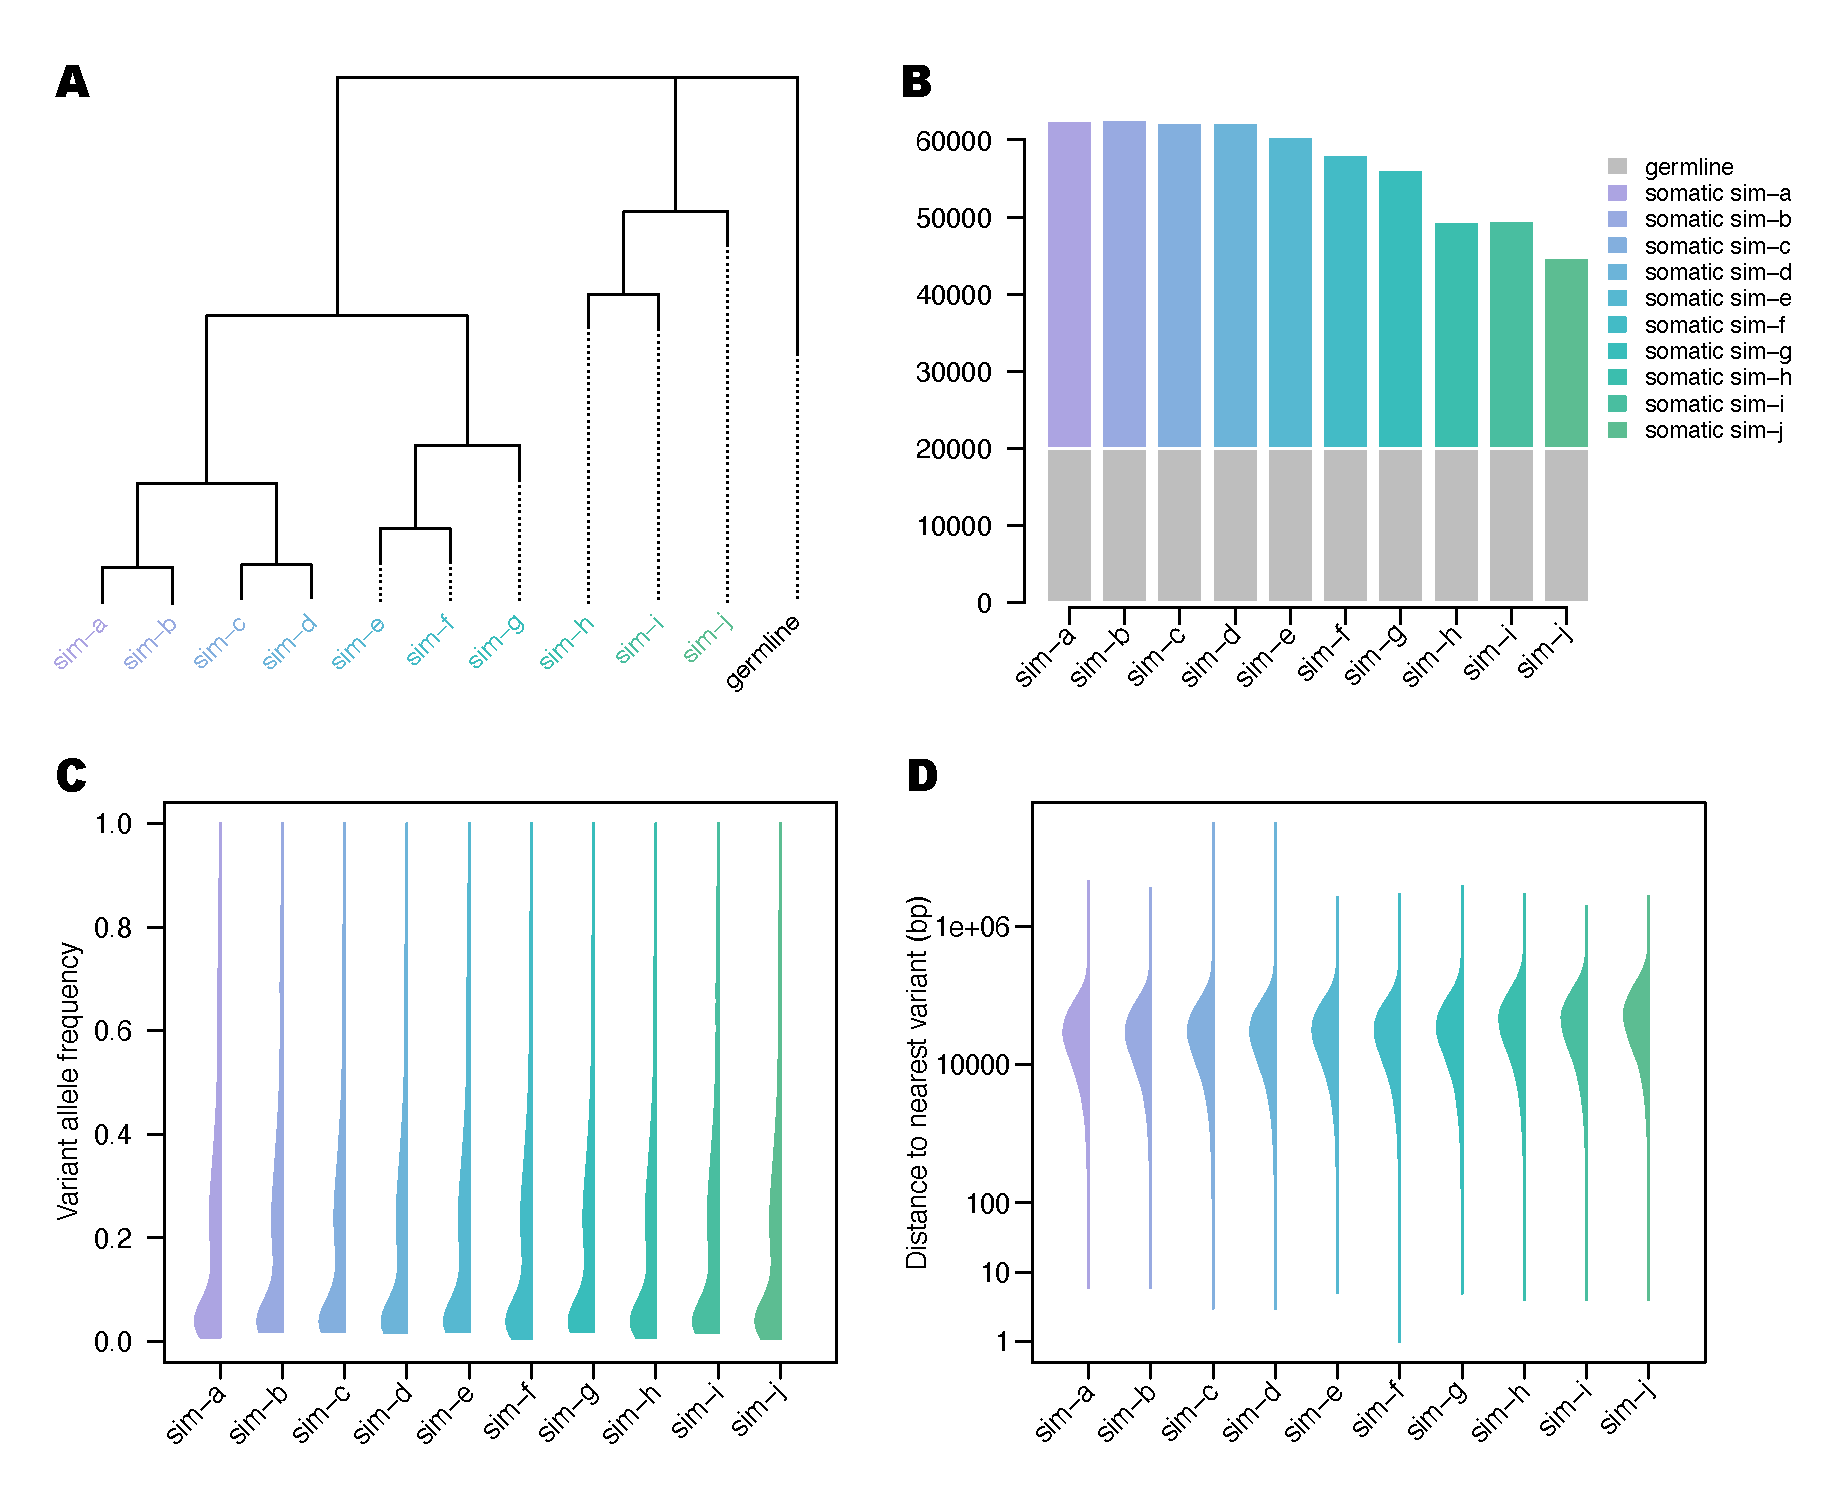
\includegraphics[width=\textwidth]{Appendices/Variantcalling/supp/S1}
  \caption[Characteristics of simulated data]{Characteristics of simulated data: A) Simulated phylogeny of samples B) Number of simulated germline and somatic variants per sample C) Variant allele frequency distribution of simulated variants per sample D) Distance to nearest variant in each sample.}\label{A:fig:S01}
\end{figure}

\begin{figure}[!ht]
\centering
  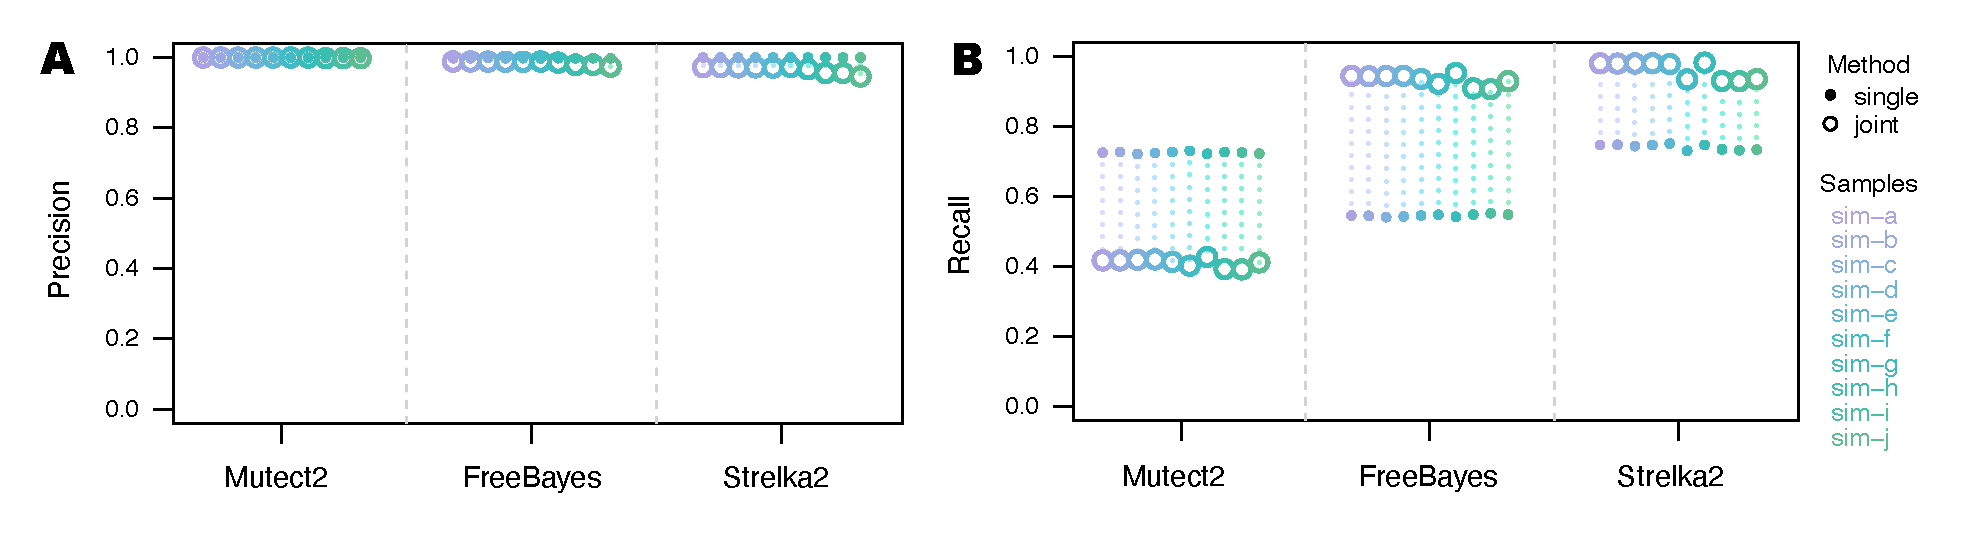
\includegraphics[width=\textwidth]{Appendices/Variantcalling/supp/S2}
  \caption[Performance of workflows using simulated data]{Performance of workflows using simulated data: A) Precision and B) Recall of Mutect2, FreeBayes and Strelka2, run in single tumour-normal paired and joint calling configurations.}\label{A:fig:S02}
\end{figure}

\begin{figure}[!ht]
\centering
  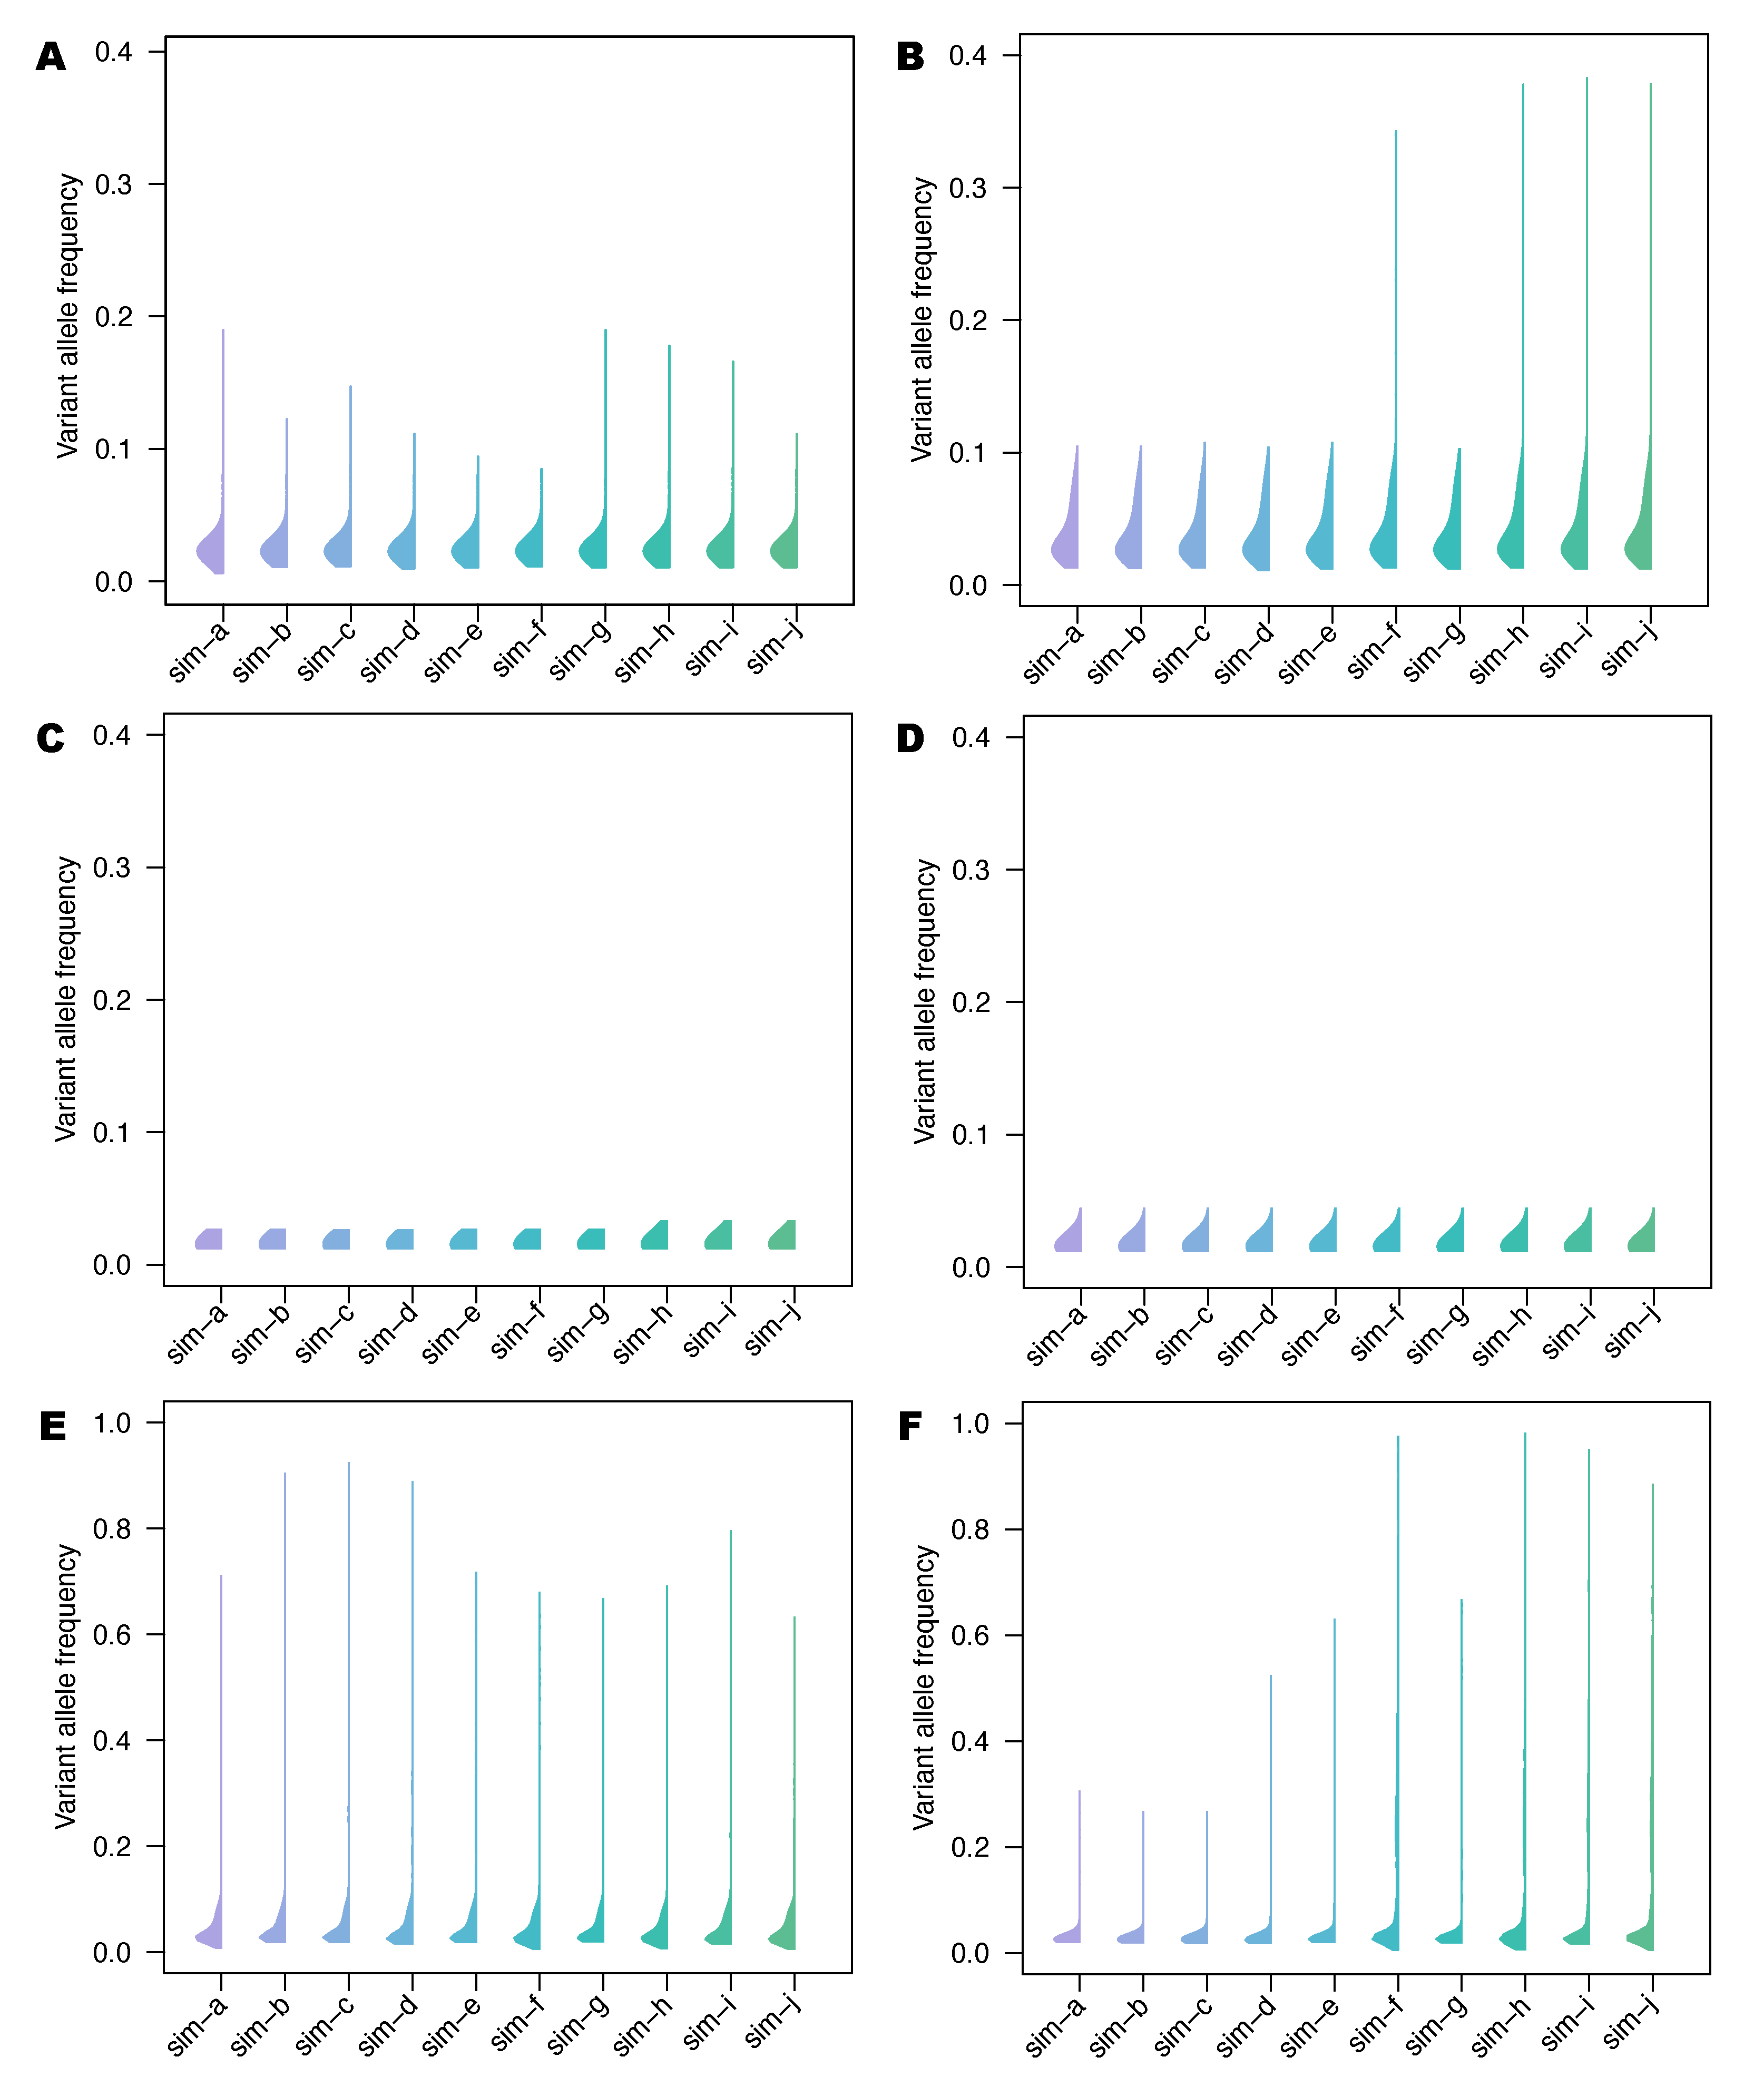
\includegraphics[width=\textwidth]{Appendices/Variantcalling/supp/S3}
  \caption[Variant allele frequencies (VAF) of variants detected by joint sample analysis]{Variant allele frequencies (VAF) of variants detected by joint sample analysis; A) VAF distribution of true positive variants additionally detected by Strelka2pass B) and FreeBayesSomatic C) VAF distribution of false positive variants additionally detected by FreeBayesSomatic D) and Strelka2pass E) VAF distribution of false negatives not called by FreeBayesSomatic F) and Strelka2pass.}\label{A:fig:S03}
\end{figure}

\begin{figure}[!ht]
\centering
  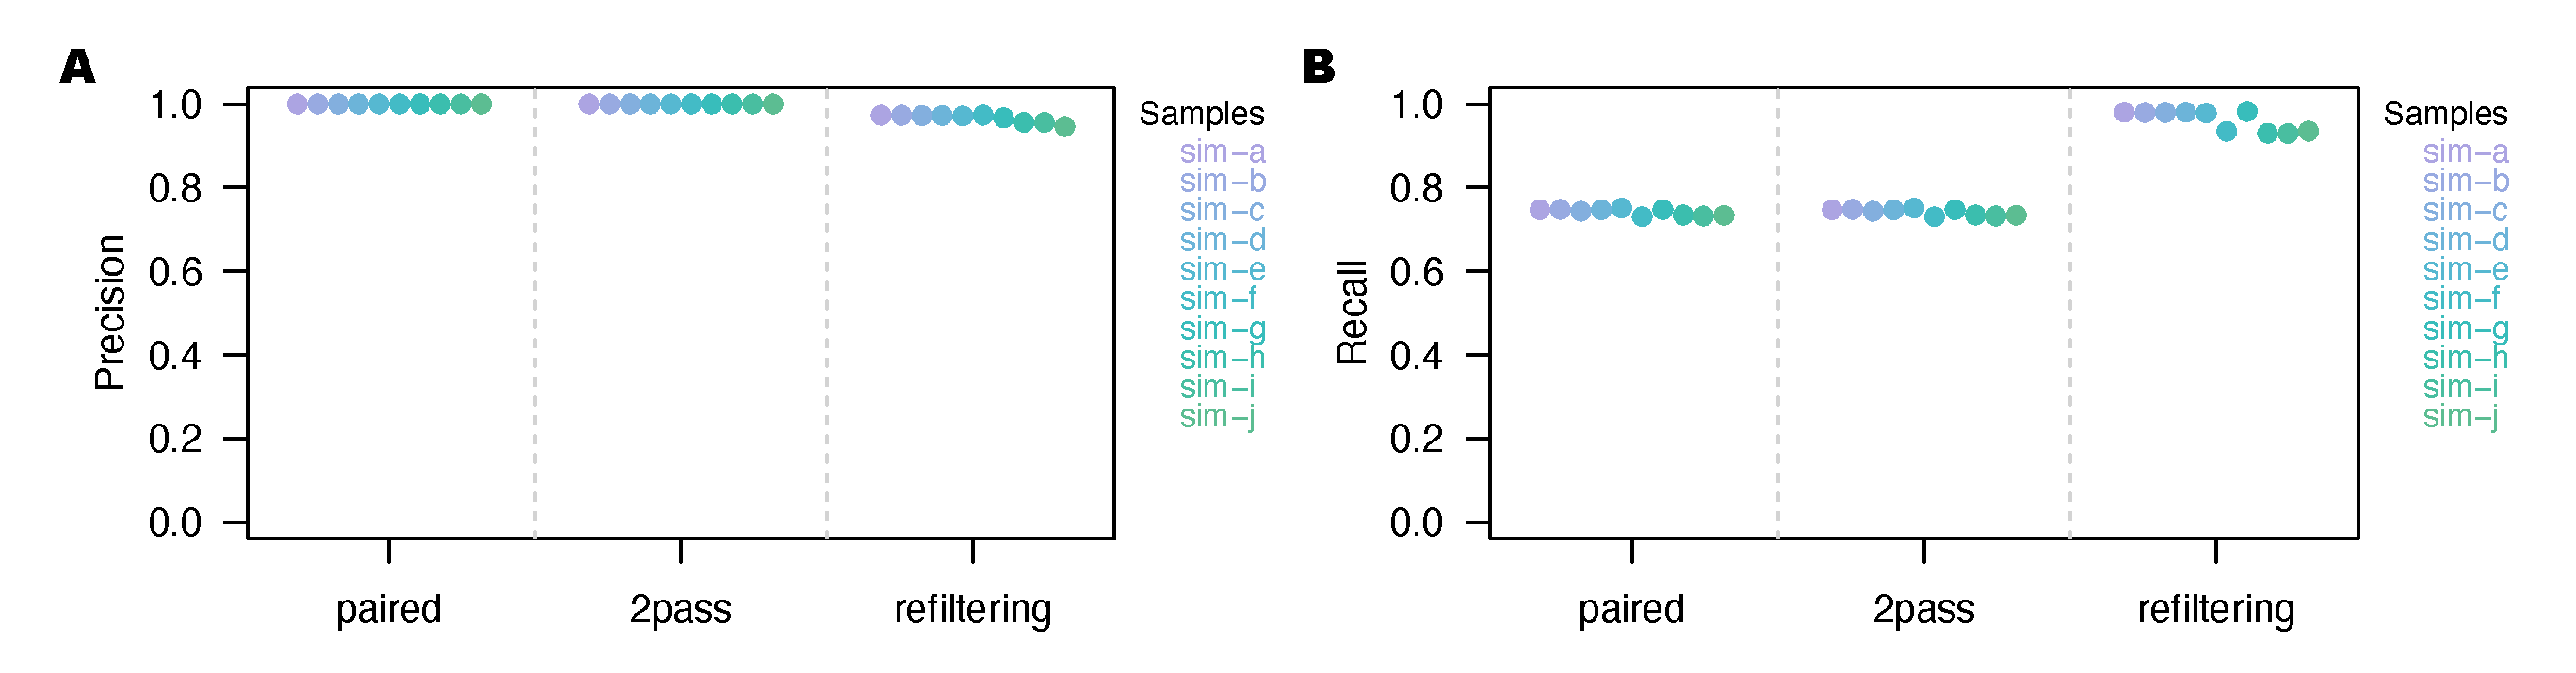
\includegraphics[width=\textwidth]{Appendices/Variantcalling/supp/S4}
  \caption[Performance of individual steps in the Strelka2pass workflow using the simulated data]{Performance of individual steps in the Strelka2pass workflow using the simulated data: A) Precision and B) Recall of tumour-normal paired analysis, two-pass step without refiltering (supplying variants from all tumour-normal pairs for evaluation) and two-pass step with refiltering (the final workflow)}\label{A:fig:S04}
\end{figure}

\begin{figure}[!ht]
\centering
  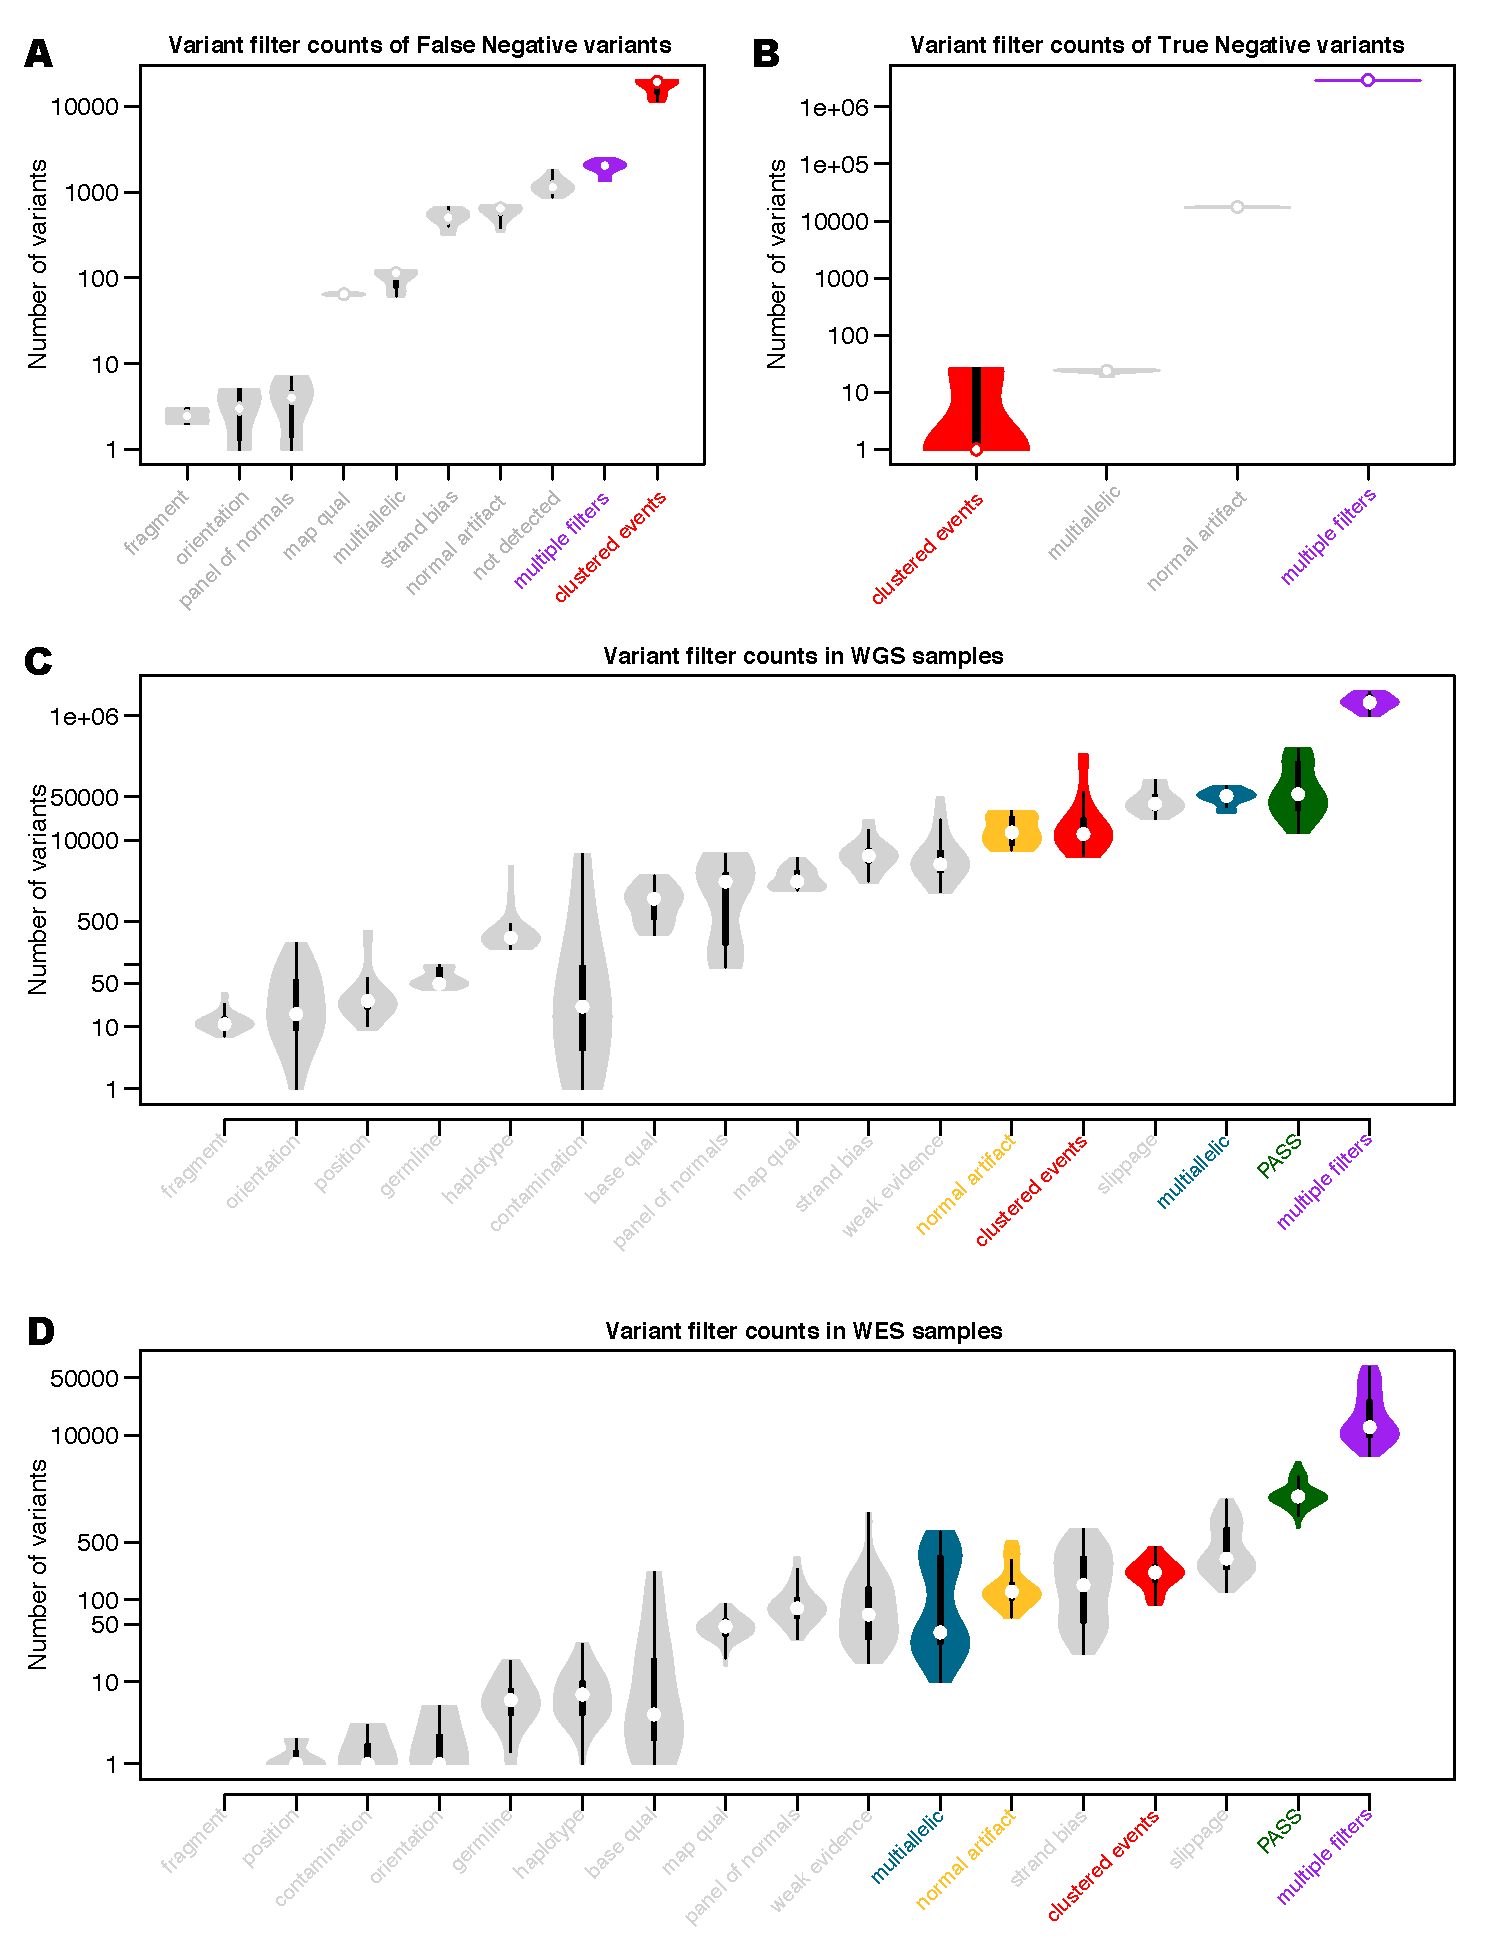
\includegraphics[width=\textwidth]{Appendices/Variantcalling/supp/S5}
  \caption[Summary of variant filters assigned by Mutect2]{Summary of variant filters assigned by Mutect2; The counts for each filter type are denoted by black boxplots with white circles depicting the median values. The fitted distribution of variant counts outlines each boxplot; A) Counts of filter assignments for false negative variants and B) true negative variants called by Mutect2 C) Filter assignment for all variants reported for sequenced patient data sequenced with WGS or D) WES.}\label{A:fig:S05}
\end{figure}

\begin{figure}[!ht]
\centering
  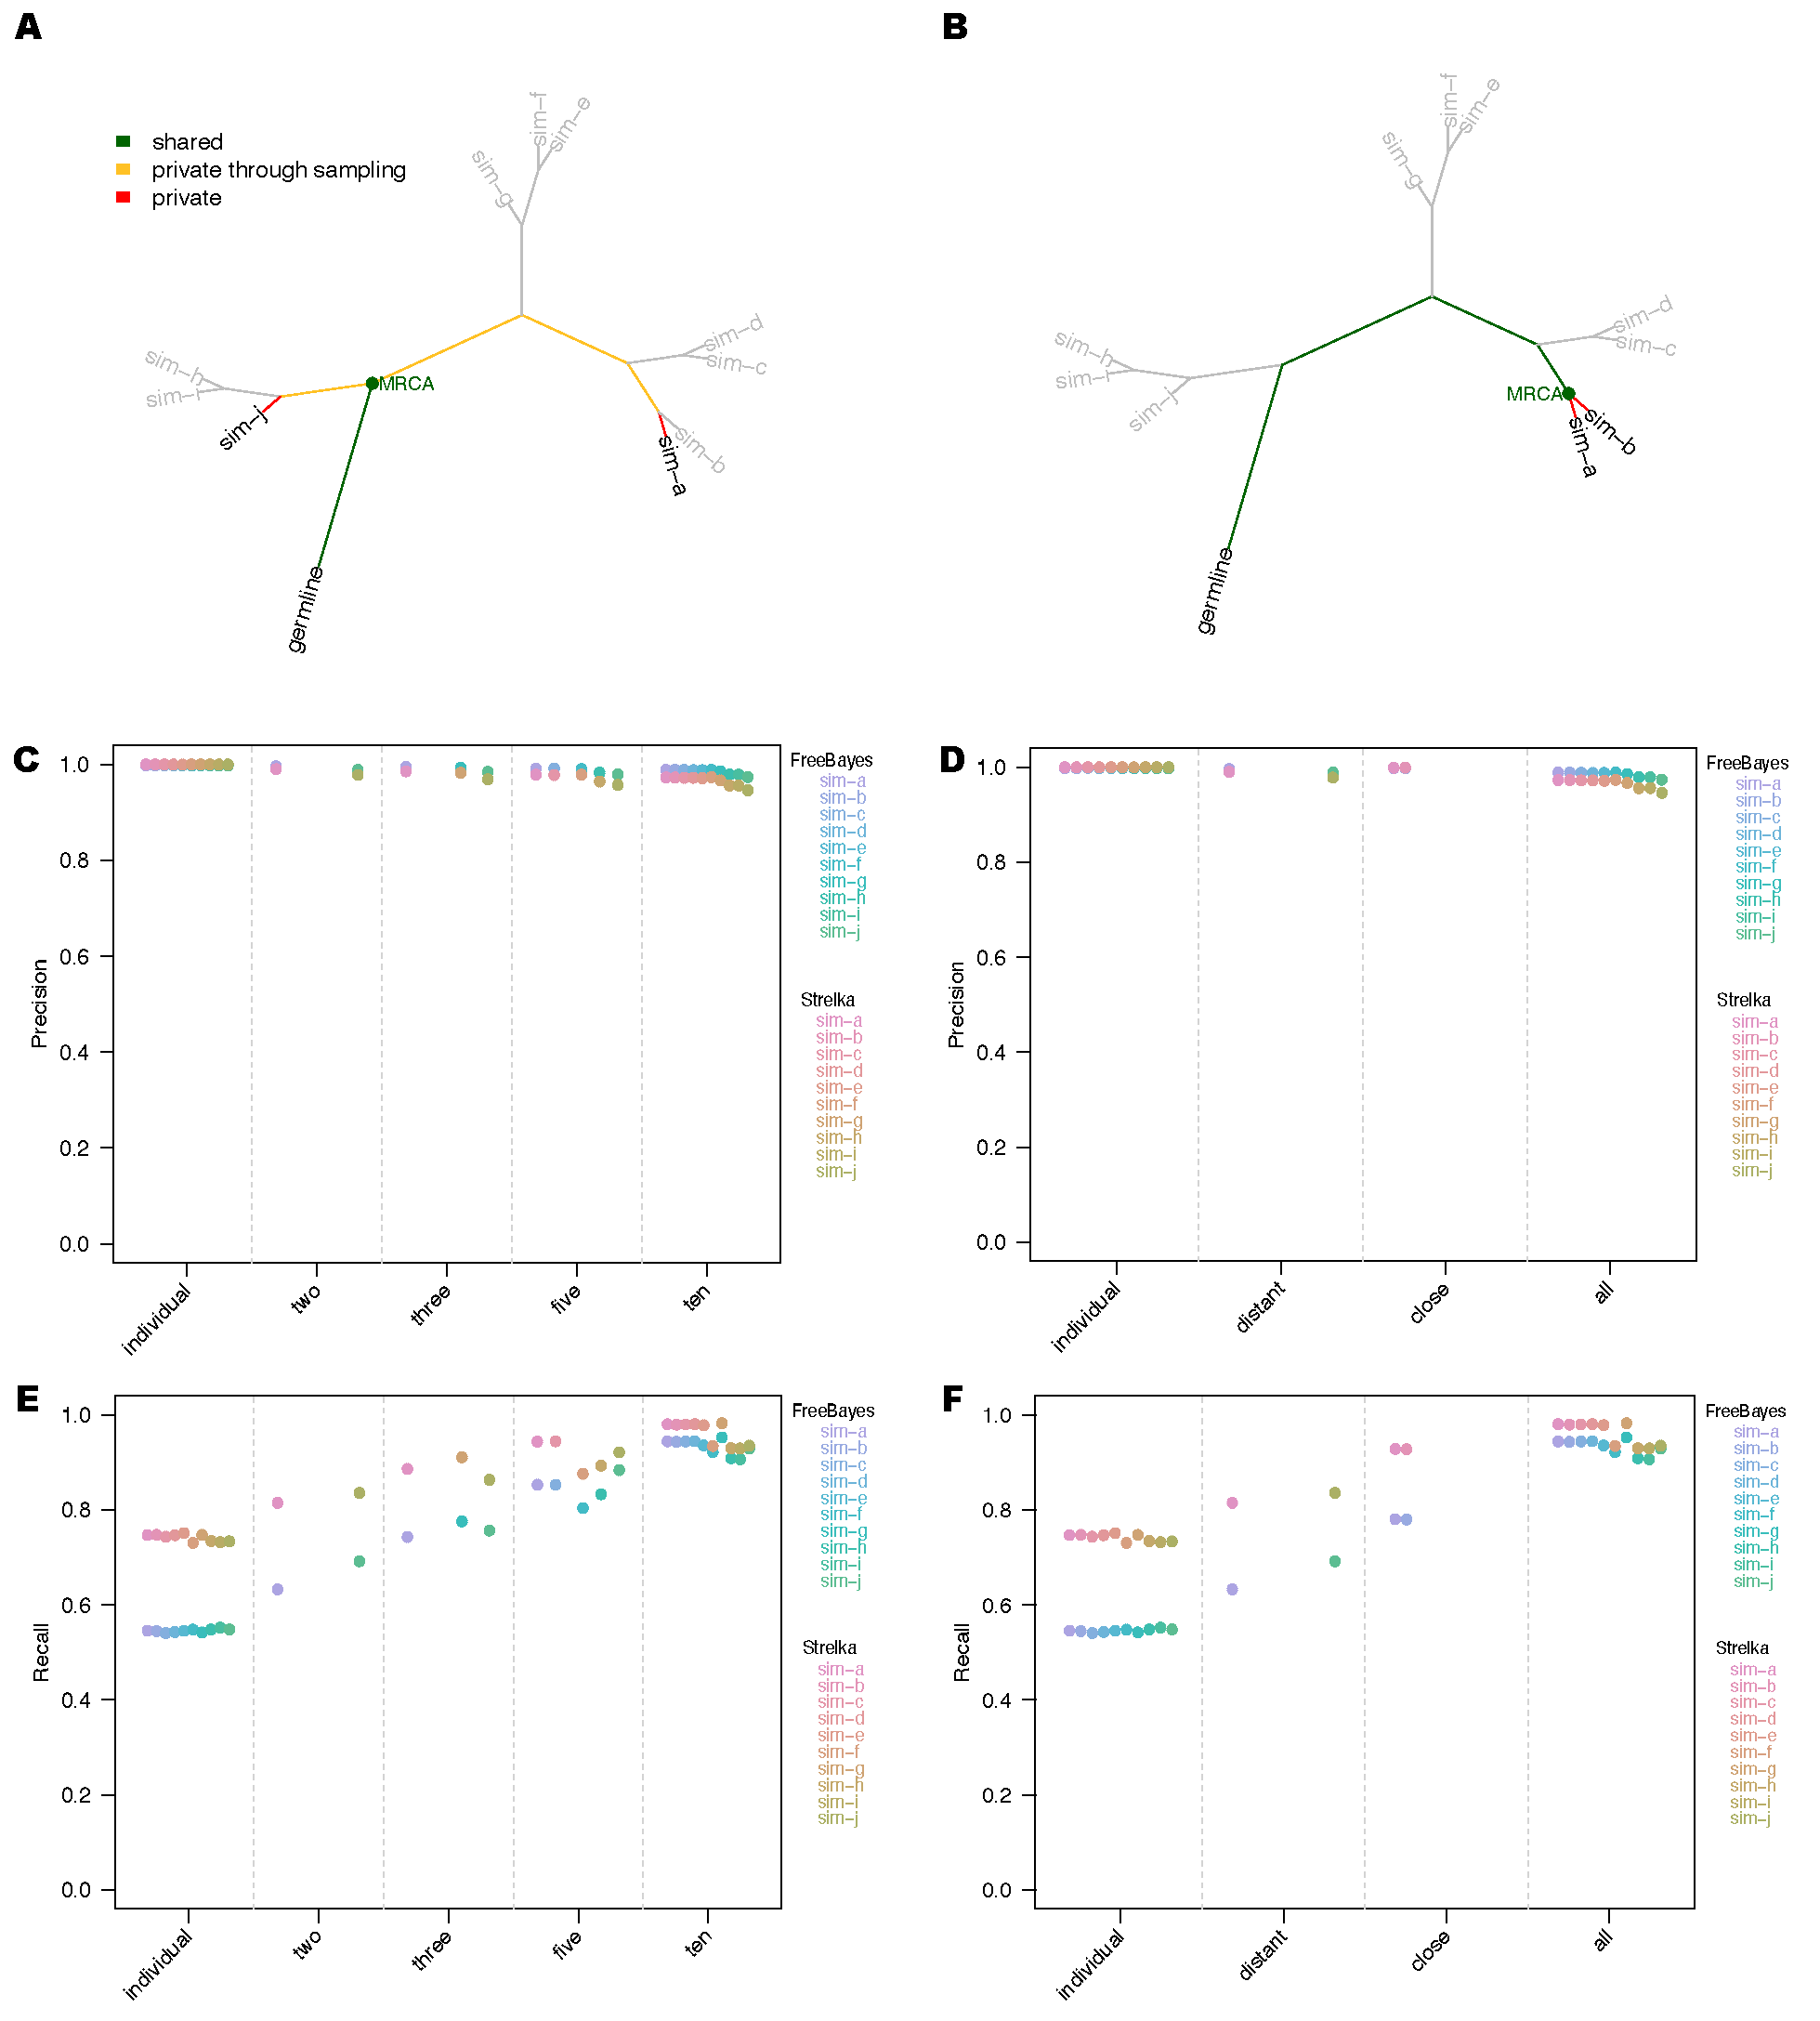
\includegraphics[width=\textwidth]{Appendices/Variantcalling/supp/S6}
  \caption[Assessing the performance of different workflows using tumour samples with different evolutionary relationships in the simulated data]{Assessing the performance of different workflows using tumour samples with different evolutionary relationships in the simulated data; A) Simulated phylogeny highlighting two samples with high evolutionary distance (sim-a and sim-j) where MRCA denotes the most recent common ancestor. B) Precision and C) Recall estimates of FreeBayes and Strelka, run in individual tumour-normal paired and joint calling configurations using two (sim-a and sim-j), three (sim-a, sim-g and sim-j), five (sim-a, sim-c, sim-f, sim-h and sim-j) and all ten tumour samples D) Simulated phylogeny highlighting two samples with low evolutionary distance (sim-a and sim-b). E) Precision and F) Recall estimates for FreeBayes and Strelka run in individual tumour-normal paired and joint calling configurations. The plots compare the performance of these workflows when using two evolutionary distant samples (sim-a and sim-j), two evolutionary close samples (sim-a and sim-b) and all ten tumour samples.}\label{A:fig:S06}
\end{figure}


\begin{figure}[!ht]
\centering
  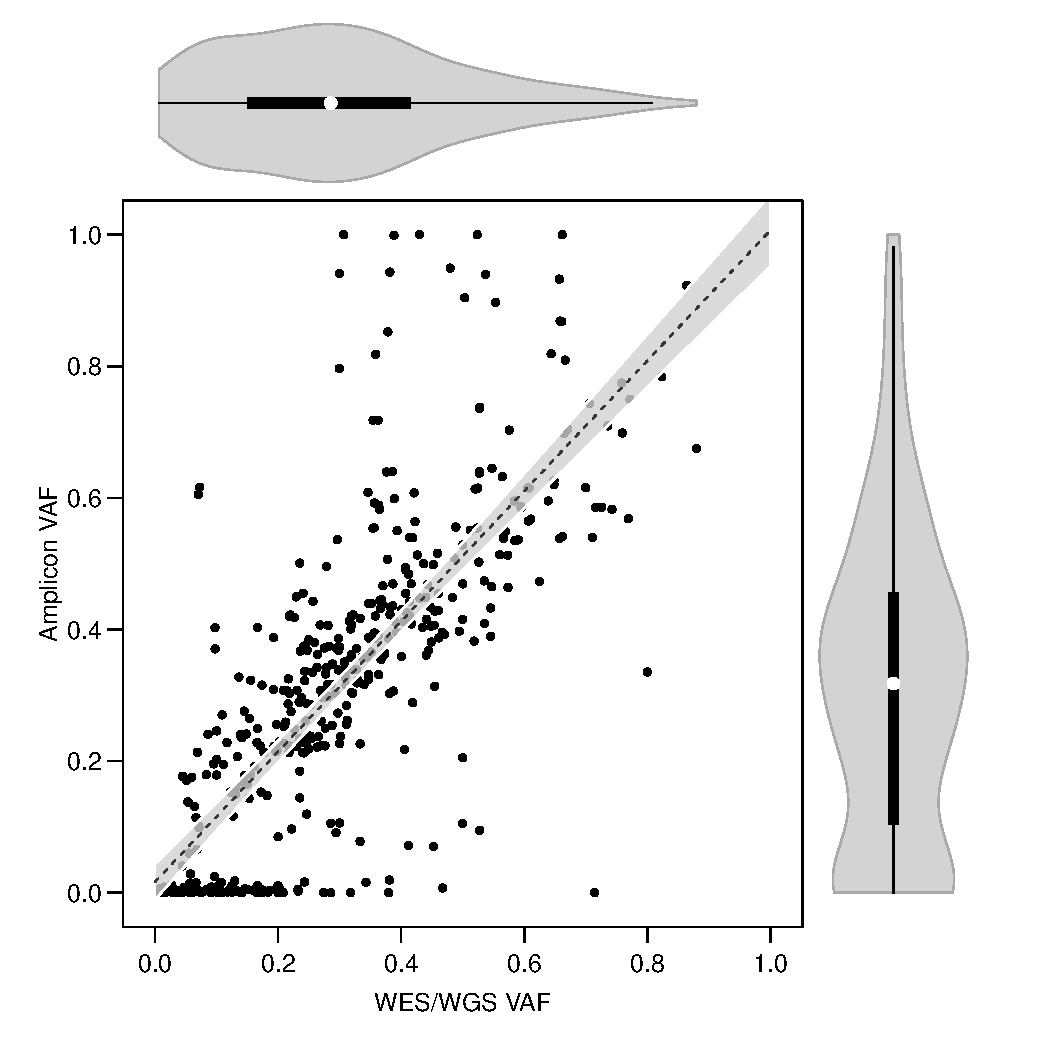
\includegraphics[width=\textwidth]{Appendices/Variantcalling/supp/S7}
  \caption[Correlation of variant allele frequencies in validation]{Correlation of variant allele frequencies (VAF) from WES and WGS data against targeted amplicon sequencing VAF values with fitted violin plots of each individual distribution. Grey background shows 95\% confidence interval for the fit of the linear model (dotted line).}\label{A:fig:S07}
\end{figure}

\begin{figure}[!ht]
\centering
  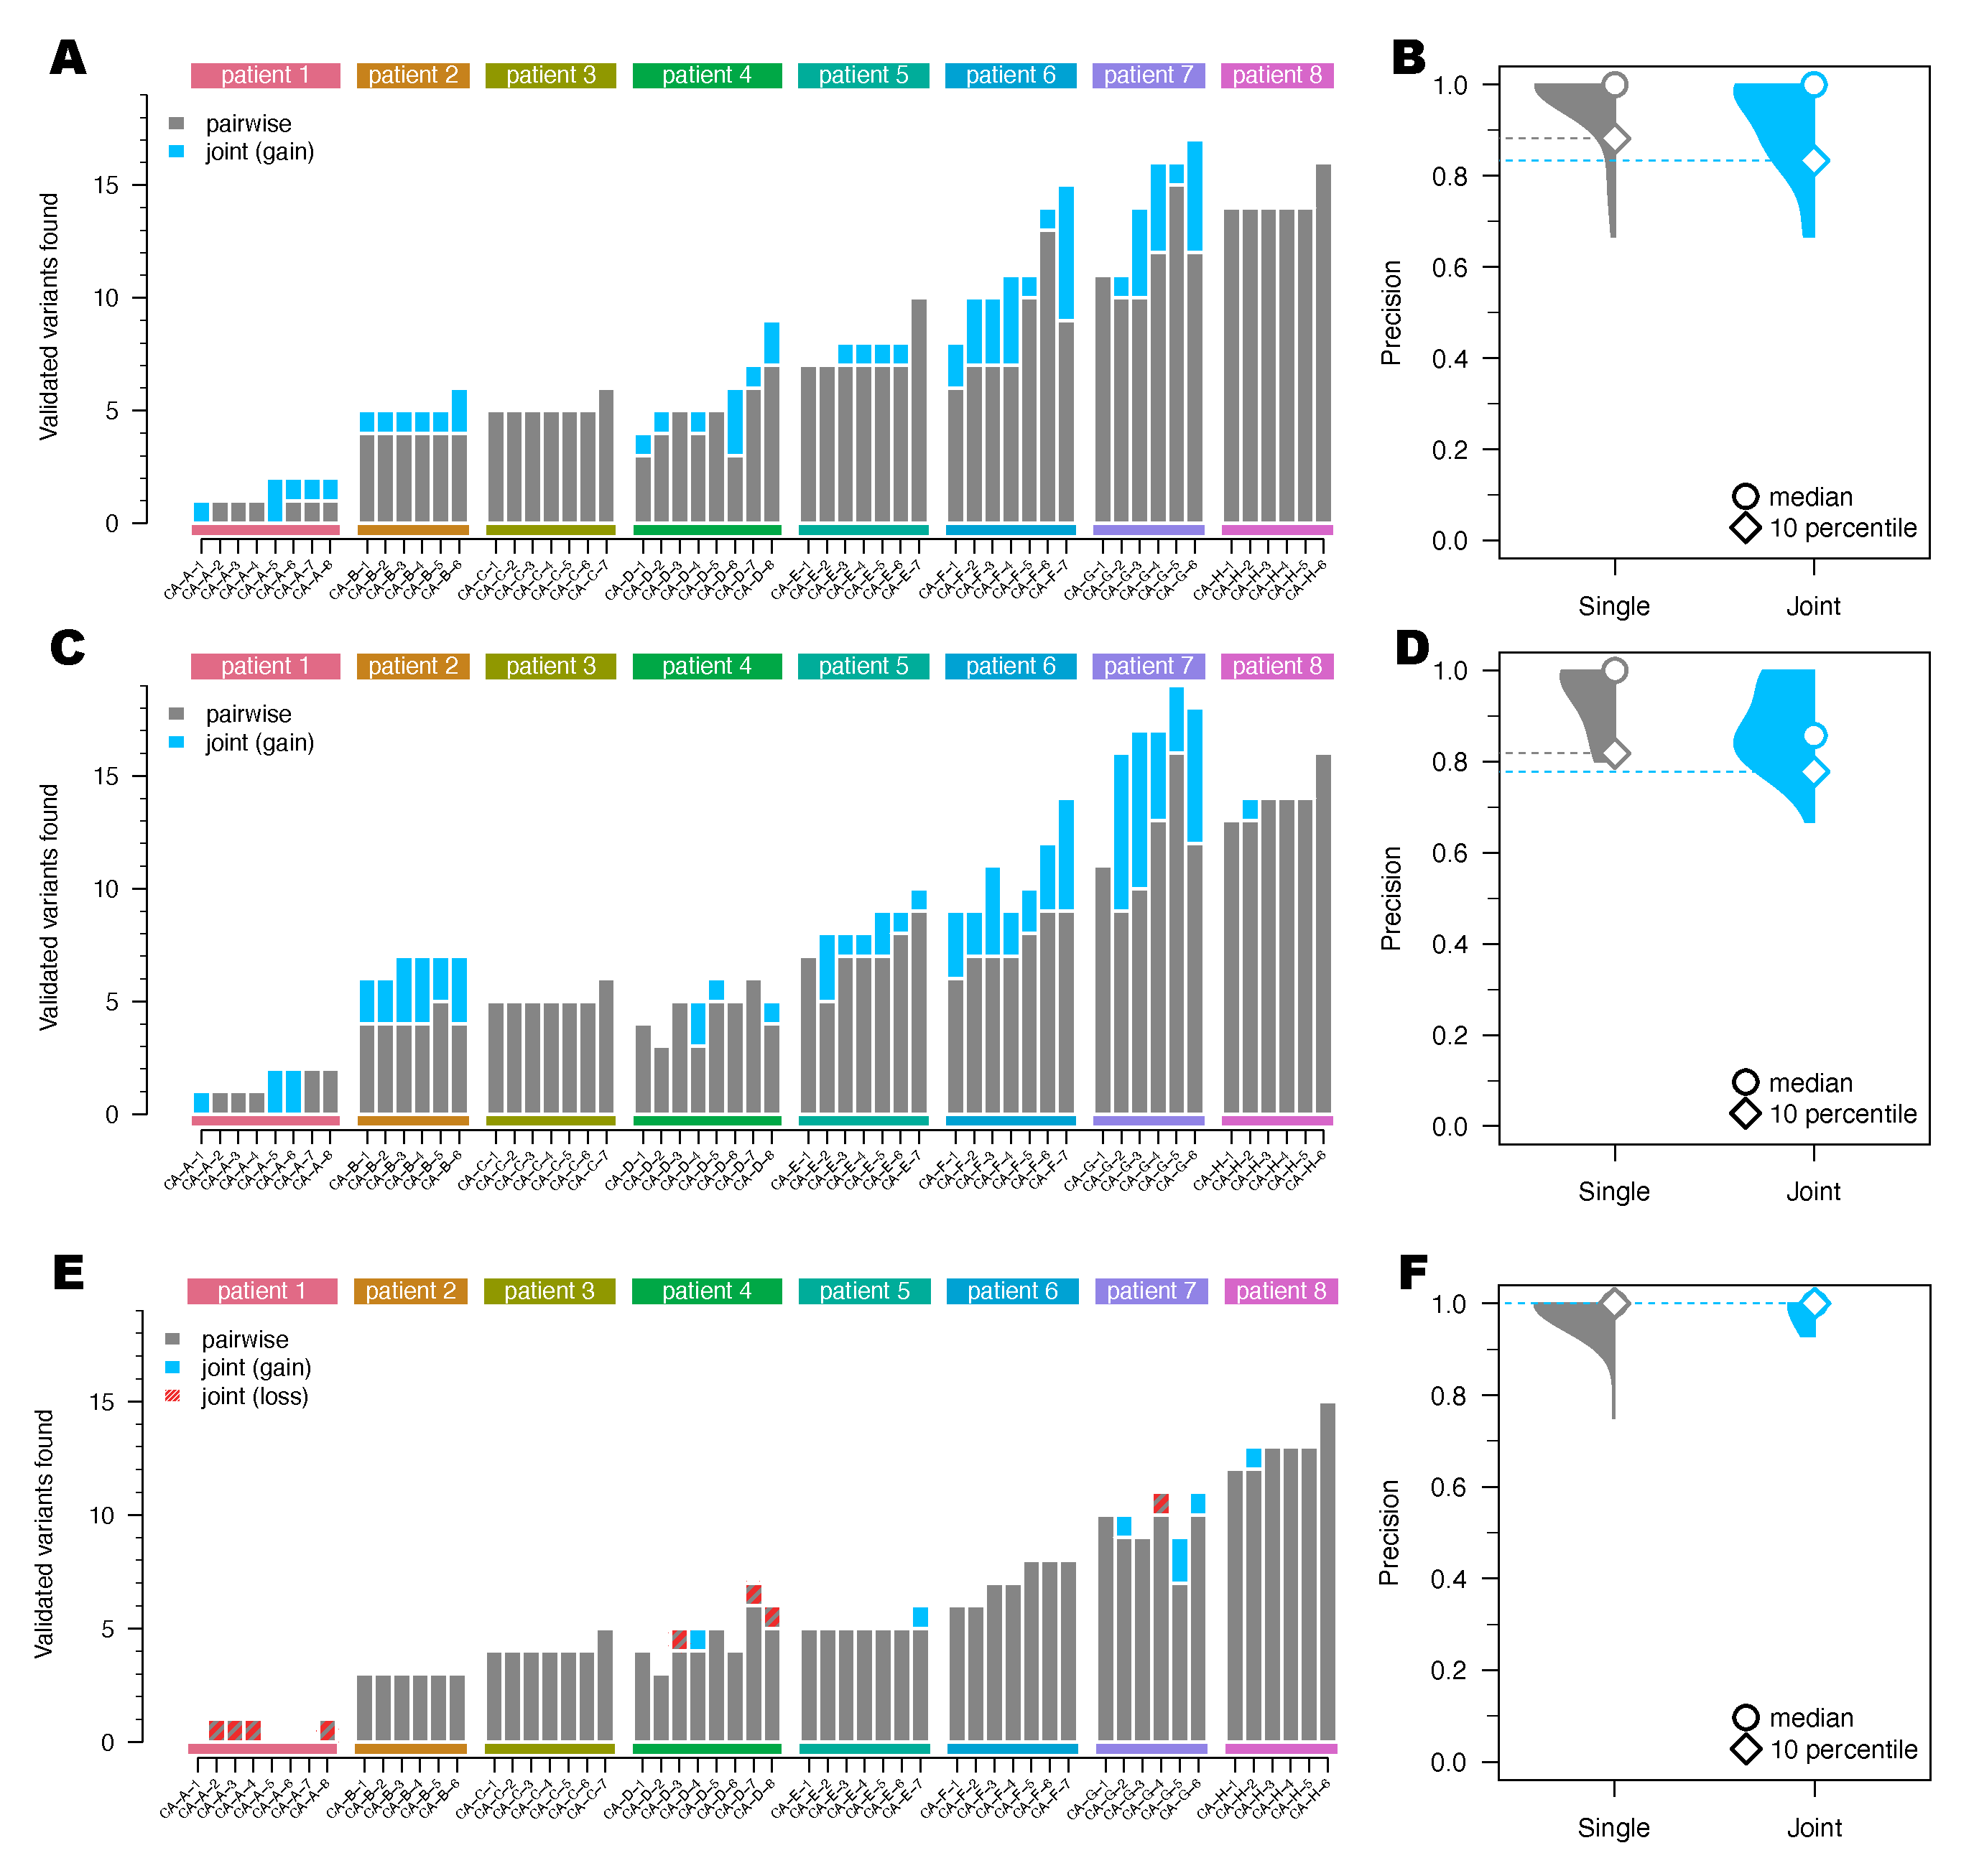
\includegraphics[width=\textwidth]{Appendices/Variantcalling/supp/S8}
  \caption[Performance of the different workflows using clinical samples from eight cancer patients]{Performance of the different workflows using clinical samples from eight cancer patients: A) Number of variants called by Strelka2 run in the tumour-normal paired (grey) and joint calling configurations, which have been validated by targeted amplicon sequencing (TAS). The same for C) FreeBayes and E) Mutect2 workflows. Precision of tumour-normal paired and joint analysis of TAS validated clinical data for B) Strelka2, D) FreeBayes and F) Mutect2; Sup. Table 1 provides the sample naming map to the original publications.}\label{A:fig:S08}
\end{figure}

\begin{figure}[!ht]
\centering
  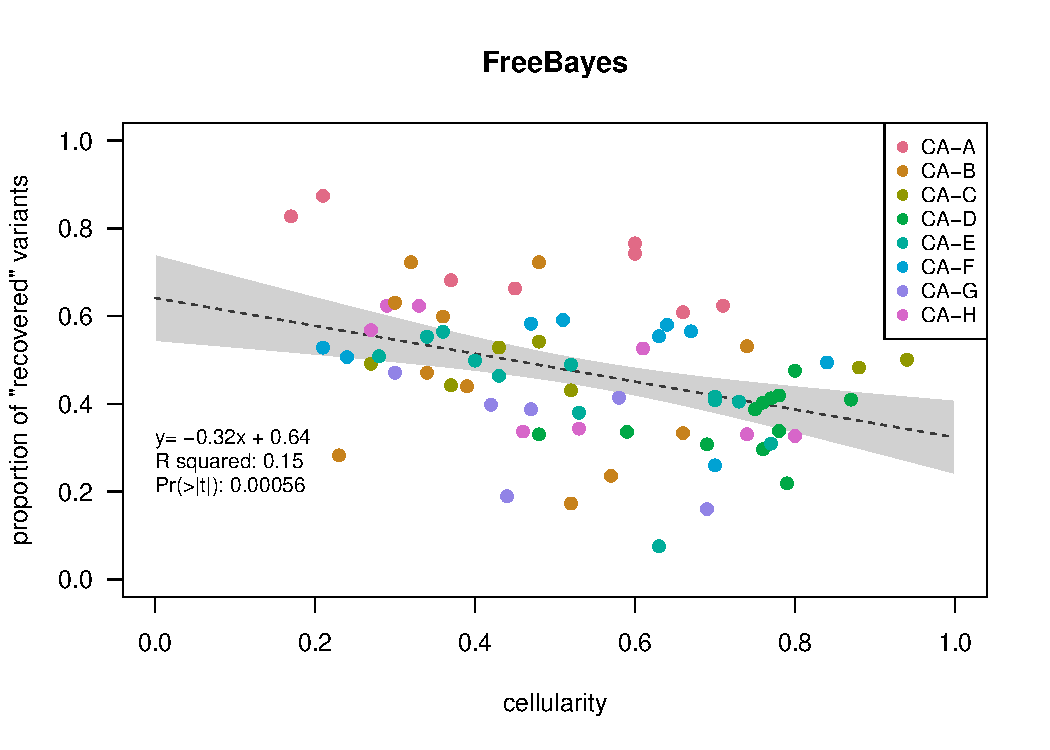
\includegraphics[width=\textwidth]{Appendices/Variantcalling/supp/S9}
  \caption[Correlation between cellularity and proportion of variants found only with joint calling using FreeBayesSomatic]{Correlation between cellularity and proportion of variants found only with joint calling using FreeBayesSomatic. Grey background shows 95\% confidence interval for fit of linear model (dotted line)}\label{A:fig:S09}
\end{figure}

\begin{figure}[!ht]
\centering
  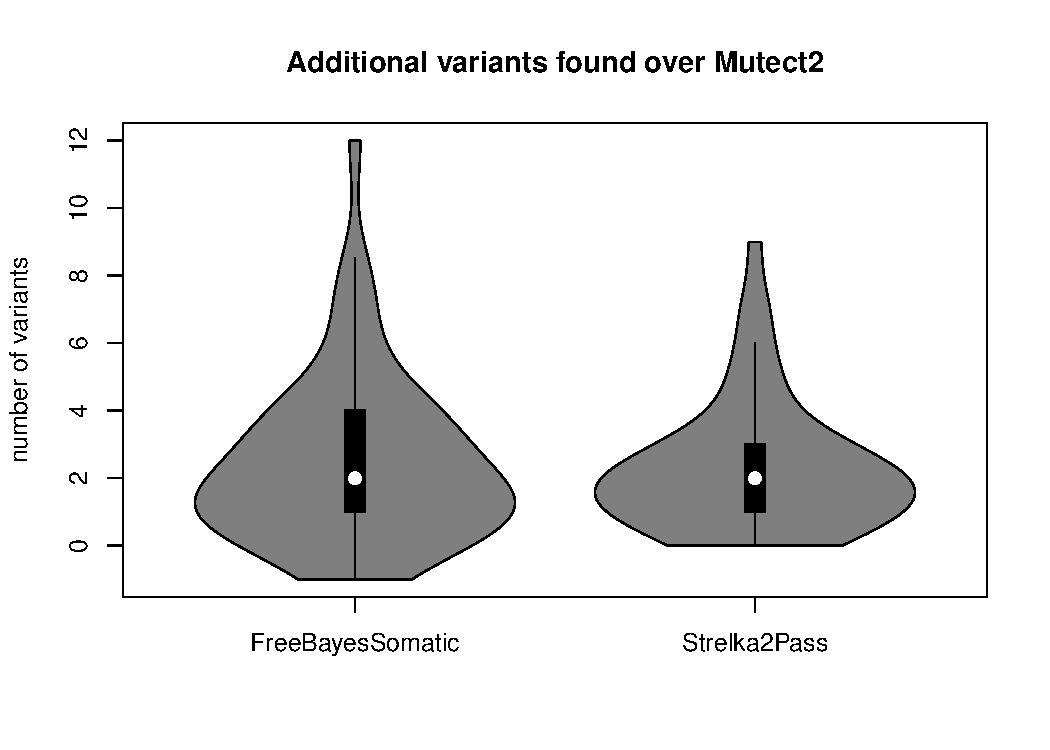
\includegraphics[width=\textwidth]{Appendices/Variantcalling/supp/S10}
  \caption{Improvement in recall using FreeBayesSomatic and Strelka2pass over Mutect2 in the clinical samples.}\label{A:fig:S10}
\end{figure}

\begin{figure}[!ht]
\centering
  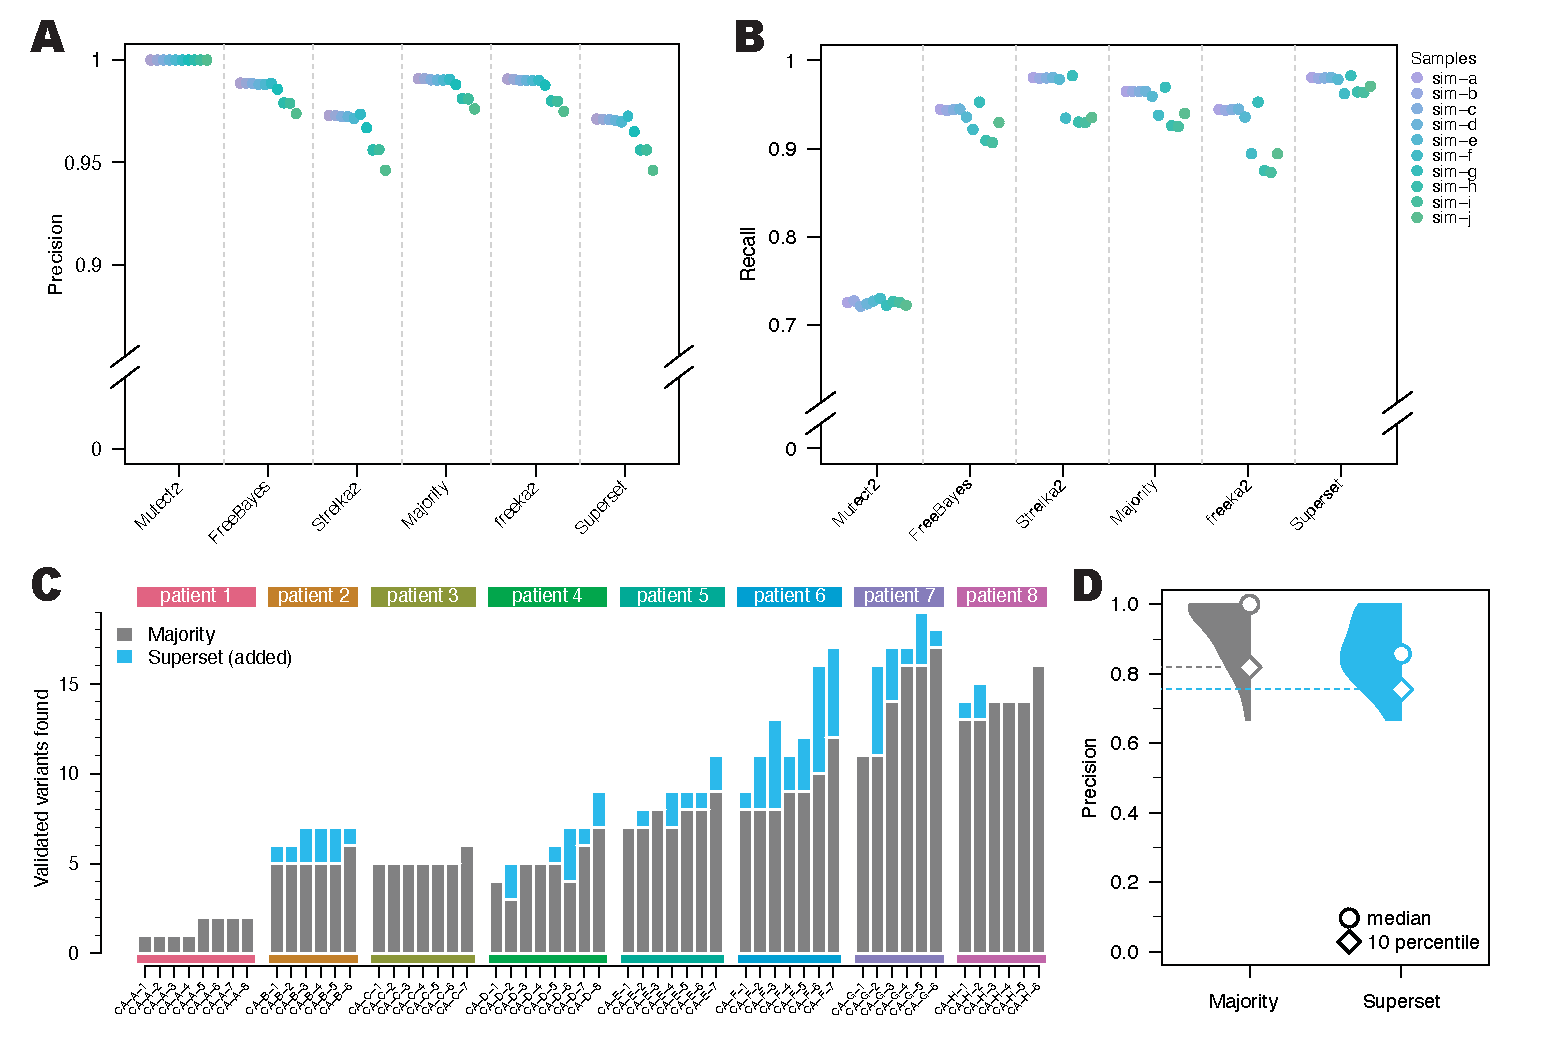
\includegraphics[width=\textwidth]{Appendices/Variantcalling/supp/S11}
  \caption[Performance of ensemble variant calling strategies]{Performance of ensemble variant calling strategies. A) Precision and B) Recall of variant detection using the joint multi-sample calling of each tool separately and compared to using Majority-vote ensemble calling (variant is called by at least two callers), Freeka2 (variant is called by both FreeBayesSomatic and Strelka2pass) and Superset (variant is called by either FreeBayesSomatic or Strelka2pass) for the simulated dataset D) Number of TAS validated variants found in the clinical samples with Majority-vote and Superset methods and the corresponding D) Precision estimates.}\label{A:fig:S11}
\end{figure}


\begin{table}[!ht]
\caption[Sample name mapping]{Sample naming map relating to previously published datasets. The first column contains sample names as they appear in this work, and the third column denotes how the samples are referred to in the original studies. Forth column shows the type of sequencing WES: whole-exome sequencing; WGS: whole genome sequencing.}\label{A:tab:S1}
\centering
%wont fit this on the page otherwise
\footnotesize
\rowcolors{2}{white}{gray!15}
\begin{tabular}{c|c|l|c}
\toprule
\textbf{SAMPLE NAME} & \textbf{PUBLISHED STUDY} & \textbf{ORIGINAL NAME} & \textbf{SEQUENCING TYPE} \\
\midrule
CA-A-1	&  \cellcolor{white} & Case 1 Left liver 1	& \cellcolor{green!9}\\
CA-A-2	& \cellcolor{white} &	Case 1 Right occipital & \cellcolor{green!9}\\
CA-A-3	& \cellcolor{white} &	Case 1 Right liver 2	 & \cellcolor{green!9}\\
CA-A-4	& \cellcolor{white} &	Case 1 Right pleura	 & \cellcolor{green!9}\\
CA-A-5	& \cellcolor{white} &	Case 1 Left lower lung lobe	 & \cellcolor{green!9}\\
CA-A-6	& \cellcolor{white} &	Case 1 Left liver 5	 & \cellcolor{green!9}\\
 CA-A-7	& \cellcolor{white} &	Case 1 Right liver 3	 & \cellcolor{green!9}\\
CA-A-8	& \cellcolor{white} \multirow{-8}{*}{\citeauthor*{Solomon2020} \cite{Solomon2020}} &	Case 1 Left liver 2	 &  \cellcolor{green!9}\multirow{-8}{*}{WGS}\\
\hhline{-|-|-|-}
CA-B-1 &  \cellcolor{white} &CAS-B-21-L-LUNG & \cellcolor{blue!9}\\ 
CA-B-2 &  \cellcolor{white} &CAS-B-22-R-LUNG	& \cellcolor{blue!9} \\ 
CA-B-3 &  \cellcolor{white} &CAS-B-14B37035-1B & \cellcolor{blue!9} \\ 
CA-B-4 &  \cellcolor{white} &CAS-B-Primary-1 & \cellcolor{blue!9} \\ 
CA-B-5 &  \cellcolor{white} &CAS-B-15B08317-3A & \cellcolor{blue!9} \\ 
CA-B-6 &  \cellcolor{white} &CAS-B-14B37035-1C & \cellcolor{blue!9}\multirow{-6}{*}{WES} \\ 
\hhline{-|~|-|-}
CA-C-1 &  \cellcolor{white} &CAS-A-FR07935894 & \cellcolor{green!9} \\ 
CA-C-2 &  \cellcolor{white} &CAS-A-FR07935905 & \cellcolor{green!9} \\ 
CA-C-3 &  \cellcolor{white} &CAS-A-FR07935906 & \cellcolor{green!9} \\ 
CA-C-4 &  \cellcolor{white} &CAS-A-FR07935907 & \cellcolor{green!9} \\ 
CA-C-5 &  \cellcolor{white} &CAS-A-FR07935908 & \cellcolor{green!9} \\ 
CA-C-6 &  \cellcolor{white} &CAS-A-FR07935916 & \cellcolor{green!9} \\ 
CA-C-7 &  \cellcolor{white} &CAS-A-FR07935918 & \cellcolor{green!9}\multirow{-7}{*}{WGS} \\ 
\hhline{-|~|-|-}
CA-D-1 &  \cellcolor{white} &CAS-G-91-2 & \cellcolor{blue!9}\\ 
CA-D-2 &  \cellcolor{white} &CAS-G-75 & \cellcolor{blue!9} \\ 
CA-D-3 &  \cellcolor{white} &CAS-G-74 & \cellcolor{blue!9} \\ 
CA-D-4 &  \cellcolor{white} &CAS-G-71 &  \cellcolor{blue!9}\\ 
CA-D-5 &  \cellcolor{white} &CAS-G-91 &  \cellcolor{blue!9}\\ 
CA-D-6 &  \cellcolor{white} &CAS-G-76 & \cellcolor{blue!9} \\ 
CA-D-7 &  \cellcolor{white} &CAS-G-94 & \cellcolor{blue!9} \\ 
CA-D-8 &  \cellcolor{white} &CAS-G-72 & \cellcolor{blue!9}\multirow{-8}{*}{WES}\\ 
\hhline{-|~|-|-}
CA-E-1 &  \cellcolor{white} &CAS-D-70 & \cellcolor{blue!9}\\ 
CA-E-2 &  \cellcolor{white} &CAS-D-61-3 & \cellcolor{blue!9} \\ 
CA-E-3 &  \cellcolor{white} &CAS-D-66 & \cellcolor{blue!9} \\ 
CA-E-4 &  \cellcolor{white} &CAS-D-68 & \cellcolor{blue!9} \\ 
CA-E-5 &  \cellcolor{white} &CAS-D-64 &  \cellcolor{blue!9}\\ 
CA-E-6 &  \cellcolor{white} &CAS-D-61-2 &  \cellcolor{blue!9}\\ 
CA-E-7 &  \cellcolor{white} &CAS-D-62 & \cellcolor{blue!9} \multirow{-7}{*}{WES}\\ 
\hhline{-|~|-|-}
CA-F-1 &  \cellcolor{white} &CAS-C-41 & \cellcolor{blue!9}\\ 
CA-F-2 &  \cellcolor{white} &CAS-C-40-Fresh & \cellcolor{blue!9} \\ 
CA-F-3 &  \cellcolor{white} &CAS-C-37 & \cellcolor{blue!9} \\ 
CA-F-4 &  \cellcolor{white} &CAS-C-44 & \cellcolor{blue!9} \\ 
CA-F-5 &  \cellcolor{white} &CAS-C-42-Fresh & \cellcolor{blue!9} \\ 
CA-F-6 &  \cellcolor{white} &CAS-C-43-Fresh & \cellcolor{blue!9} \\ 
CA-F-7 &  \cellcolor{white} &CAS-C-46-Primary & \cellcolor{blue!9} \multirow{-7}{*}{WES}\\ 
\hhline{-|~|-|-}
CA-G-1 &  \cellcolor{white} &CAS-F-FR07935922 & \cellcolor{green!9}\\ 
CA-G-2 &  \cellcolor{white} &CAS-F-FR07935915 & \cellcolor{green!9} \\ 
CA-G-3 &  \cellcolor{white} &CAS-F-FR07935913 & \cellcolor{green!9} \\ 
CA-G-4 &  \cellcolor{white} &CAS-F-FR07935909 & \cellcolor{green!9} \\ 
CA-G-5 &  \cellcolor{white} &CAS-F-FR07935904 & \cellcolor{green!9} \\ 
CA-G-6 &  \cellcolor{white} &CAS-F-FR07935903 & \cellcolor{green!9}\multirow{-6}{*}{WGS} \\ 
\hhline{-|~|-|-}
CA-H-1 &  \cellcolor{white} &CAS-E-1 & \cellcolor{blue!9}\\ 
CA-H-2 &  \cellcolor{white} &CAS-E-3 & \cellcolor{blue!9} \\ 
CA-H-3 &  \cellcolor{white} &CAS-E-4 & \cellcolor{blue!9} \\ 
CA-H-4 &  \cellcolor{white} &CAS-E-10 & \cellcolor{blue!9} \\ 
CA-H-5 &  \cellcolor{white} &CAS-E-6 & \cellcolor{blue!9} \\ 
CA-H-6 & \cellcolor{white}\multirow{-47}{*}{\citeauthor*{Vergara2021} \cite{Vergara2021}} & CAS-E-8 & \cellcolor{blue!9} \multirow{-6}{*}{WES}\\ 
\bottomrule
\end{tabular}
\end{table}

%get rid of all the floats we accumulated
\clearpage

\begin{table}[!ht]
\caption[Runtime of different workflows on simulated data]{Runtime of different workflows on simulated data; The runtimes were generated on the Peter MacCallum Cancer Centre HPC cluster with Intel(R) Xeon(R) CPU E5-2660 v3 @ 2.60GHz. The times are displayed in single CPU runtime, but each workflow is highly parallelised, such that the user runtime is far lower.}\label{A:tab:S2}
\centering
\begin{tabular}{r | R{0.12\textwidth} | R{0.12\textwidth} | R{0.12\textwidth} | R{0.12\textwidth} |}
\toprule
 & \multicolumn{4}{c}{\textbf{Number of tumour samples used for joint calling}}\\
 \cline{2-5}
 \textbf{Method} & 2 & 3 & 5 & 10 \\
 \hline\hline
 \rowcolor{gray!15}
 FreeBayesSomatic & \num{562}h & \num{811}h & \num{1185}h & \num{2292}h \\
 \hline
Strelka2Pass & \num{310}h & 	\num{465}h & \num{776}h & \num{1552}h \\
 \hline
 \rowcolor{gray!15}
Mutect2 & - & - & - & \num{28418}h \\
 \hline
 \bottomrule
\end{tabular}
\end{table}



\section{Supplementary methods}
\label{A:varcalling:supmethods}
\subsection{Alignment of clinical data}
Detailed information on processing of the clinical sequencing datasets was published previously \cite{Solomon2020,Vergara2021}. Briefly, reads were aligned to GRCh38 for patient CAS-A and GRCh37 for patients CAS-B through CAS-H using BWA version 0.7.17 \cite{Li2009} allowing the use of alternative contigs. Reads were then marked as duplicates with Picard software (v2.17.3). 

\subsection{Validation of clinical data}
\label{A:varcalling:clinical}
Detailed information on targeted amplicon sequencing of patient samples can be found in the original publications \cite{Solomon2020,Vergara2021}. A SNV called in WES with any workflow was considered a true positive when the adjusted p-value calculated through an exact binomial test was lower than 0.05 on the TAS data. The probability of success for this test was estimated as the number of bases different from the reference divided by the total number of sequenced bases (0.001) and the number of trials was the read depth covering the variant. For indels, a variant was considered to be validated if either of the panel variant callers primal (in house) or canary \cite{Doig2017} called the same variant. 

Only amplicons with an average mapping rate of at least 80\% over all samples, as well as an average coverage of more than 300 were considered for further analysis. WES variants were first subsetted to be within the area of the respective amplicons.

\subsection{Purity estimation with sequenza}
For CA-A the sequenza-utils python program was used to generate input files for the sequenza R program on the aligned BAM files \cite{Favero2015}. Kmin and gamma were set to 100 and 500 respectively to discourage a highly fragmented result.  For CA-B through -H the reported tumour purities were used from the publication \cite{Vergara2021}.

\subsection{Performance of individual steps in Strelka2Pass}
\label{A:varcalling:steps}
As each of the three steps potentially has implications for the performance, we assessed the improvement provided by each step in the Strelka2pass workflow. \autoref{A:fig:S04} shows, that there is no change in either precision or recall just by supplying variants from all tumour-normal pairs for a second round of evaluation. However, there is a >20\% improvement in recall when coupling this to the refiltering step that we have built into the workflow. 

\subsection{Ensemble workflows – user suggestions}
An overall workflow can contain any number of additional variant callers, when not restricted to callers with joint analysis capability. Importantly, there is no benefit of jointly analysing samples with Mutect2, and it may decrease the performance in some cases. Each of our presented workflows outperformed Mutect2 on the data shown here, so when assembling an ensemble method, these methods, should have a higher confidence assigned to them in joint analysis cases, than tumour-normal pair approaches.

Depending on the end needs of the user, an ensemble workflow can be optimised towards precision or recall. In \autoref{A:fig:S11} we show the performance changes improvement that can be achieved by combining Mutect2 in tumour-normal paired analysis with the two new workflows FreeBayesSomatic and Strelka2Pass. First, in a “best of three” majority vote, where the variant needs to be called by two out of three variant callers, we enhance the precision of each of the individual tools, with slightly lower recall.
On the other hand, with the super set approach, where any variant called in either FreeBayesSomatic or Strelka2Pass is included in the end result, this improves the recall even further, but slightly reduces the precision. This approach has the additional benefit of not needing to run Mutect2 which is an order of magnitude slower in our tests, than Strelka2Pass and FreeBayesSomatic (\autoref{A:tab:S2}).
The usage of these workflows can be easily integrated into existing workflows and  can be customised to the needs of the user.



%reset this to what we had before
\fancyhead[RO]{\rightmark}